% =====================================================================
%  SmartGarage: Automatic Vehicle Inspection and Service System Using OpenGL
%  Project report (showcase / viva edition) - Afifa Sultana Offa, Roll 2107087
%  Build:  latexmk -pdf main.tex   (or pdflatex, bibtex, pdflatex, pdflatex)
% =====================================================================
\documentclass[10pt,a4paper]{article}

\usepackage[T1]{fontenc}
\usepackage[utf8]{inputenc}
\usepackage{lmodern}
\usepackage{microtype}
\usepackage{graphicx}
\usepackage{amsmath,amssymb}
\usepackage{booktabs,longtable,array,tabularx}
\usepackage{float}
\usepackage{caption,subcaption}
\usepackage{geometry}
\usepackage[table]{xcolor}
\usepackage{listings}
\usepackage{tikz}
\usetikzlibrary{arrows.meta,calc,positioning,shapes.geometric}
\usepackage{siunitx}
\usepackage{fancyhdr}
\usepackage{enumitem}

\usepackage[hidelinks]{hyperref}

\geometry{left=0.75in,right=0.75in,top=0.65in,bottom=0.65in}
\setlength{\parindent}{0pt}
\setlength{\parskip}{3pt}
\setlength{\emergencystretch}{3em}
\setlength{\textfloatsep}{7pt plus 2pt minus 2pt}
\setlength{\floatsep}{5pt plus 2pt minus 2pt}
\setlength{\intextsep}{5pt plus 2pt minus 2pt}
\setlength{\abovedisplayskip}{9pt plus 3pt minus 3pt}\setlength{\belowdisplayskip}{9pt plus 3pt minus 3pt}\setlength{\jot}{5pt}
\renewcommand{\topfraction}{0.92}\renewcommand{\bottomfraction}{0.8}
\renewcommand{\textfraction}{0.06}\renewcommand{\floatpagefraction}{0.85}
\setlist{itemsep=2pt,topsep=2pt,parsep=0pt}
\captionsetup{font=small,labelfont=bf,skip=3pt}
\captionsetup[sub]{font=footnotesize,labelfont=bf,skip=1pt}
\renewcommand{\arraystretch}{1.0}
\setcounter{tocdepth}{1}
\setcounter{secnumdepth}{2}

\pagestyle{fancy}\fancyhf{}
\fancyfoot[C]{\footnotesize\thepage}
\renewcommand{\headrulewidth}{0pt}

\lstset{language=C++, basicstyle=\ttfamily\scriptsize, backgroundcolor=\color{gray!7},
  keywordstyle=\color{smcyan!55!black}\bfseries, commentstyle=\color{smsteel}\itshape,
  frame=single, rulecolor=\color{smsteel!60}, breaklines=true, columns=fullflexible,
  aboveskip=3pt, belowskip=3pt, morekeywords={vec3,uniform,out,reflect,normalize,mix,pow,dot,max}}

\newcommand{\fn}[1]{\texttt{#1}}
\newcommand{\vect}[1]{\mathbf{#1}}
\newcommand{\shot}[2]{\includegraphics[width=#1]{#2}}
% Implementation card: Object | File | Function | Variables = values | Effect of a change | Equation / evidence
\newcommand{\viva}[6]{\par\smallskip\noindent\fcolorbox{smcyan}{smcyan!5}{\begin{minipage}{\dimexpr\linewidth-2\fboxsep-2\fboxrule\relax}\scriptsize
\textbf{\textcolor{smcyan!50!black}{IMPLEMENTATION CARD}} \textbf{--- #1} \hfill \textbf{File:} #2\\
\textbf{Function:} #3\\
\textbf{Variables = current values:} #4\\
\textbf{If changed:} #5\\
\textbf{Equation / evidence:} #6\end{minipage}}\par\smallskip}

\definecolor{smcyan}{HTML}{25A9C4}
\definecolor{smamber}{HTML}{D9A525}
\definecolor{smsteel}{HTML}{6F777D}
\definecolor{smhead}{HTML}{E3E1DA}
\let\oldtoprule\toprule
\renewcommand{\toprule}{\oldtoprule\rowcolor{smhead}}

\begin{document}
% ------------------------------------------------------------------ title page
\begin{titlepage}
\newcommand{\cfs}[2]{\fontsize{#1}{#2}\selectfont}
\centering
\vspace*{0.1cm}
{\cfs{17}{22}\bfseries CSE 4102: Computer Graphics and Image Processing\par}\vspace{0.7cm}
{\cfs{18}{22}\bfseries PROJECT REPORT\par}\vspace{0.15cm}
{\cfs{13}{16}\bfseries ON\par}\vspace{0.4cm}
\rule{0.80\textwidth}{0.7pt}\par\vspace{0.35cm}
{\cfs{20}{26}\bfseries SmartGarage: Automatic Vehicle Inspection\\[2pt] and Service System Using OpenGL\par}\vspace{0.3cm}
\rule{0.80\textwidth}{0.7pt}\par\vspace{0.55cm}
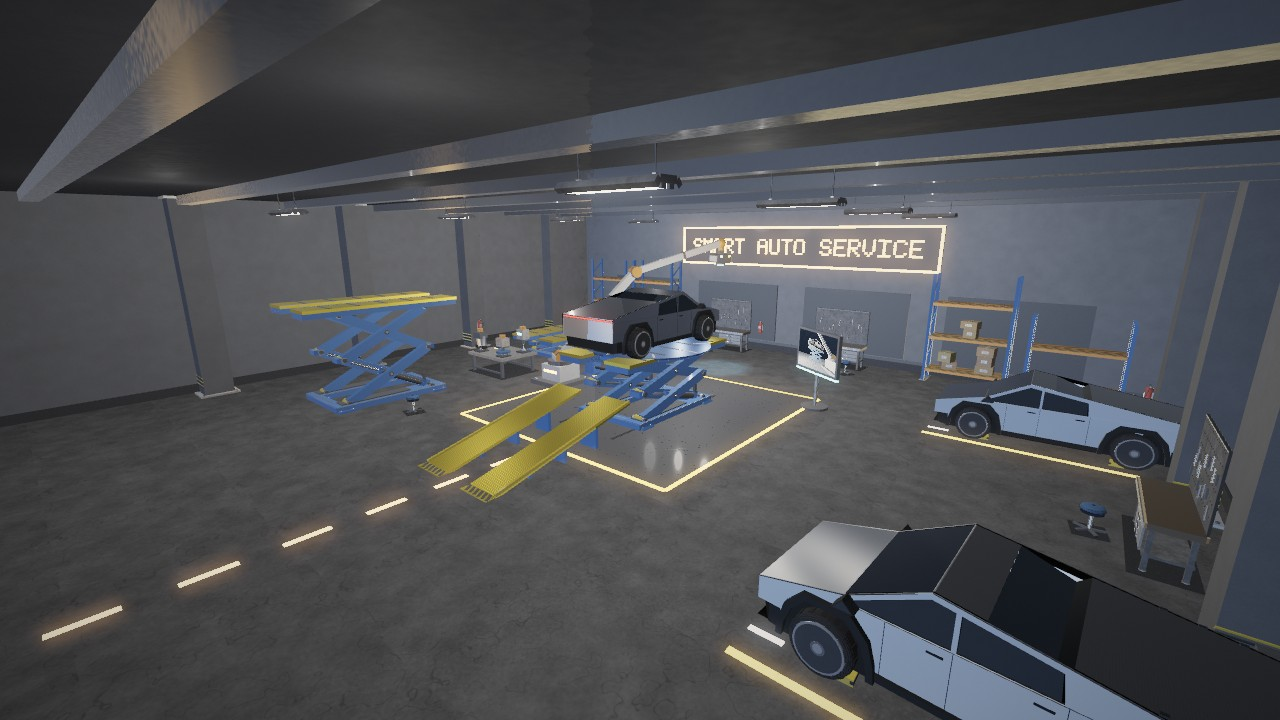
\includegraphics[width=0.70\textwidth]{images/garage/garage_overview.jpg}\par\vspace{0.8cm}
\noindent\hspace*{0.02\textwidth}\begin{minipage}[t]{0.60\textwidth}\raggedright
{\cfs{19}{23}\bfseries Submitted To\par}\vspace{0.45cm}
{\cfs{18}{22}\bfseries Md. Tajmilur Rahman\par}\vspace{0.12cm}
{\cfs{16}{20}\bfseries Lecturer\par}\vspace{0.55cm}
{\cfs{18}{22}\bfseries Md. Mubtashim Abrar Nihal\par}\vspace{0.12cm}
{\cfs{16}{20}\bfseries Lecturer\par}
\end{minipage}%
\begin{minipage}[t]{0.38\textwidth}\raggedright
{\cfs{19}{23}\bfseries Submitted By\par}\vspace{0.45cm}
{\cfs{18}{22}\bfseries Afifa Sultana Offa\par}\vspace{0.2cm}
{\cfs{17}{21}\bfseries Roll: 2107087\par}
\end{minipage}\par
\vspace{0.7cm}
{\cfs{16}{20}\bfseries Submission Date: October 7, 2026\par}
\vfill
{\cfs{15}{19}\bfseries Department of Computer Science and Engineering\\[2pt]
Khulna University of Engineering \& Technology\\[2pt]
Khulna 9203, Bangladesh\par}
\vspace*{0.1cm}
\end{titlepage}
\setcounter{page}{2}

% ------------------------------------------------------------------ abstract + contents
\section*{Abstract}
SmartGarage is an OpenGL~3.3 (core profile) application in which a Cybertruck-style vehicle waits outside a smart
service garage, the roller door opens, the vehicle drives in and climbs a ramp onto a scissor lift, the door closes,
the lift rises, and a five-joint robotic arm inspects the vehicle with a moving spotlight, cleans and polishes it,
tightens the wheel fasteners, and finally the lift lowers, the door opens and the vehicle reverses out. The whole
sequence is an 18-state machine lasting \SI{197.7}{s}. Every object is built in code from a reusable cube, two
cylinders and a sphere, except the vehicle shell, which is a custom triangle mesh. All 21 items of the original
proposal are implemented --- hierarchical modelling, transformations, directional, point, spot and moving
lights, ambient--diffuse--specular lighting, \textbf{Gouraud} and \textbf{Phong} shading, motion and interaction ---
and are extended with Cook--Torrance PBR, shadow mapping, textures, HDR post-processing collision handling, and a physical inspection monitor whose picture is produced by genuine \emph{ray tracing} with shadow rays (the rest of the garage stays rasterised). The
report gives the real construction sequence of the vehicle, lift and robot with the calculations behind each step, an
equation and figure for every other object, and for every part its source file, variables and the effect of a change.

\smallskip\noindent\textbf{Keywords:} OpenGL, GLSL, hierarchical modelling, Phong reflection, Gouraud shading, Phong shading, animation, robotic arm.

\bigskip
\tableofcontents
\clearpage

% =====================================================================
\section{Introduction}\label{sec:intro}
\textbf{Background.} Real-time graphics renders triangles through vertex processing, rasterisation and fragment
shading~\cite{segal2010opengl,devries2020learnopengl}. SmartGarage uses one scenario --- an automated service bay ---
to demonstrate the course topics: geometry, transformation, lighting, shading, motion and interaction.

\textbf{Objectives.} (1) generate primitives procedurally and reuse them through model matrices; (2) build the
garage, vehicle, lift and robot hierarchically; (3) implement the Phong lighting model with Gouraud and Phong
shading and four light types; (4) animate the full inspection sequence; (5) let the user control the camera,
door, lift, robot, lights and shading. The six mandatory course requirements are \emph{lighting, transformation,
Gouraud shading, Phong shading, motion/animation} and \emph{interaction}; ray tracing is an optional bonus and is implemented for one dedicated view, the underbody inspection monitor of Section~\ref{sec:rt}; the rest of the garage is rasterised.

\textbf{Final concept.} Interior $28\times26\times\SI{7}{m}$ ($x\in[-14,14]$, $z\in[-13,13]$, 1 unit = 1 m); entrance
$13\times\SI{4.9}{m}$ at $z=13.2$; lift centred at $z=-2$; robot bolted at $(-4.6,0,-2.2)$; tool table at
$(-7.9,0,-1.85)$. The vehicle starts on the apron at $z=16.5$. The source is organised as \fn{Math3D.h} (maths),
\fn{Camera.h}, \fn{Primitives.cpp} (meshes), \fn{SceneObjects.cpp} (all objects), \fn{Shader.cpp} (GLSL) and
\fn{Main.cpp} (state machine, input, collision, lights, render passes); the function names are given with every
object below.

% =====================================================================
\section{Proposal-to-Final Implementation Mapping}\label{sec:proposal}
Every item of the original proposal is checked against the final source in Table~\ref{tab:proposal}; the
\textbf{Phong shading mode}, the \textbf{headlight point lights} and the \textbf{vehicle exit} were completed in
final preparation. Figures~\ref{fig:scissor}, \ref{fig:door}, \ref{fig:ramp} and \ref{fig:fsm} show the storyline rendered by the program.

{\scriptsize\setlength{\tabcolsep}{3pt}
\begin{longtable}{@{}>{\raggedright}p{2.3cm}>{\raggedright}p{2.4cm}>{\raggedright}p{4.3cm}>{\raggedright}p{3.2cm}>{\raggedright}p{1.25cm}>{\raggedright\arraybackslash}p{2.3cm}@{}}
\caption{Proposal items versus final implementation. Result: \textbf{21 of 21 implemented} (14 fully, 6 with improvement, 1 implemented differently but equivalently).}\label{tab:proposal}\\
\toprule Proposed feature & Proposal expectation & Final implementation (how) & File / function & Evidence & Status\\\midrule\endfirsthead
\toprule Proposed feature & Proposal expectation & Final implementation (how) & File / function & Evidence & Status\\\midrule\endhead
\bottomrule\endfoot
\multicolumn{6}{@{}l}{\textbf{Scene objects}}\\
Automobile & body, wheels, windows, headlights from primitives; moves in, wheels rotate & custom triangle-mesh shell (13 batches) + cylinder wheels; wheel angle $\theta=s/r$ from distance travelled & \fn{drawCar}, \fn{drawWheel}, \fn{updateCarDrive} & \ref{fig:vehicle-build} & Implemented with improvement\\
Garage entrance door & sliding door, opens / closes & 5-panel roller shutter sliding in guide rails, winding onto a drum & \fn{drawGarageDoor} & \ref{fig:door} & Implemented differently but equivalently\\
Hydraulic lift & platform moves up/down by transformation & double-scissor lift; angle solved from height, platform top $=1.08+h$ & \fn{scissorAngle}, \fn{drawHydraulicLift} & \ref{fig:lift-build} & Implemented with improvement\\
Robotic inspection arm & primitives, scanner at end; joints rotate & 5-DOF arm (yaw, shoulder, elbow, wrist pitch/roll) + 4 exchangeable tools & \fn{drawRobotArm}, \fn{runToolChange} & \ref{fig:robot-build} & Implemented with improvement\\
Inspection light fixture & spotlight on arm; ceiling lights as instances & spotlight from arm FK; 8 instances of one ceiling fixture & \fn{uploadSceneUniforms}, \fn{drawCeilingFixture} & \ref{fig:lights} & Fully implemented\\
Garage environment & floor, walls, ceiling from surfaces & scaled cubes + beams, columns, props, textured floor & \fn{drawGarage}, \fn{drawExterior} & \ref{fig:props} & Implemented with improvement\\
\multicolumn{6}{@{}l}{\textbf{Lighting design}}\\
Directional (ceiling) & fixed direction, overall light & directional key $\hat{\vect d}=(0.166,-0.922,-0.350)$ with shadow map; ceiling has 8 point lights & \fn{buildLightSpaceMatrix} & \ref{fig:lights}a & Fully implemented\\
Point light in headlights & inside each headlight, falloff & two point lights inside the front light channel, carried by the car matrix; $A=1/(1{+}0.075d{+}0.018d^2)$ & \fn{headlightLocalPosition}, \fn{uploadSceneUniforms} & \ref{fig:shading}c,d,f & Fully implemented\\
Spotlight (scanner) & mounted on arm, moves & position/direction from the wrist and tool tip every frame & \fn{robotSafetyPoints}, Shader \fn{phongReflection} & \ref{fig:shading}a,b,e & Fully implemented\\
Ambient light & base illumination & $k_aL_a=0.038$ in the Phong model; image-based ambient in PBR & \fn{phongReflection} & \ref{fig:shading} & Fully implemented\\
\multicolumn{6}{@{}l}{\textbf{Animation flow}}\\
Step 1 arrival & door opens, vehicle enters, wheels rotate, stops on lift & DOOR\_OPEN\_IN, DRIVE\_IN; ramp climb with pitch & \fn{updateServiceAutomation} & \ref{fig:ramp} & Implemented with improvement\\
Step 2 positioning & door closes, aligns & DOOR\_CLOSE; vehicle stops at $z=-2$ on the turntable & same & \ref{fig:fsm} & Fully implemented\\
Step 3 inspection & lift raises, arm scans, spotlight follows & LIFT\_UP; SCAN of 6 regions, turntable shows far side & same & \ref{fig:scissor} & Implemented with improvement\\
Step 4 lighting demo & headlights on, point lights light nearby surfaces, Gouraud vs Phong & headlights on by default (key \fn{'}); \fn{F5} cycles PBR / Gouraud / Phong & \fn{handleDiscreteKey} & \ref{fig:shading} & Fully implemented\\
Step 5 completion & lift lowers, door opens, vehicle exits & LIFT\_DOWN, DOOR\_OPEN, DRIVE\_OUT (vehicle reverses onto apron) & same & \ref{fig:fsm} & Fully implemented\\
\multicolumn{6}{@{}l}{\textbf{Interactive features}}\\
Move camera & around garage & \fn{W A S D}, \fn{Space/Ctrl}, mouse, scroll & \fn{processMovement}, \fn{Camera} & -- & Fully implemented\\
Headlights ON/OFF & toggle & key \fn{'} (light bars + point lights) & \fn{handleDiscreteKey} & \ref{fig:shading}c,f & Fully implemented\\
Control spotlight movement & move the lamp & robot keys \fn{T/G U/J I/K} move the scanner and its light & \fn{processMovement} & \ref{fig:robot} & Fully implemented\\
Rotate inspection light & manual rotation & \fn{Y/H} wrist pitch, $\leftarrow/\rightarrow$ wrist roll & same & -- & Fully implemented\\
Switch Gouraud / Phong & shading modes & \fn{F5}: PBR $\to$ Gouraud $\to$ Phong & Shader \fn{uShadingMode} & \ref{fig:shading} & Fully implemented\\
Lighting on materials & observe differences & metal / plastic / glass / rubber materials, shininess from roughness & \fn{inferMaterialType} & \ref{fig:material} & Fully implemented\\
\end{longtable}}


\textbf{Enhancements beyond the proposal:} a ray-traced underbody inspection monitor with shadow rays (Section~\ref{sec:rt}); Cook--Torrance PBR (anisotropic stainless, clear coat, image-based lighting);
directional and spot shadow maps; triplanar texture array; HDR, MSAA, bloom, ACES; perspective/orthographic switch;
cleaning, polishing and wheel service with visible tool exchange; turntable; collision prevention; B\'ezier hoses;
teaching mode showing construction stages.

% =====================================================================
\section{Object Modelling and Construction}\label{sec:objects}
\subsection{Primitive generation (how the vertices are found)}
\textbf{Cube} (\fn{kCubeVertices}): $[-0.5,0.5]^3$, 24 vertices (6 faces $\times$ 4, so each face keeps its own normal),
36 indices (2 triangles per face, e.g.\ back face $(0,1,2),(2,3,0)$, counter-clockwise from outside).

\textbf{Cylinder} (\fn{buildCylinder}, $r=0.5$, height 1, axis $y$): for boundary $i=0..N$,
\begin{equation}\theta_i=\frac{2\pi i}{N},\qquad x_i=r\cos\theta_i,\qquad z_i=r\sin\theta_i,\qquad
\vect n_i=(\cos\theta_i,0,\sin\theta_i).\label{eq:cyl}\end{equation}
\emph{Example} (project mesh $N=28$, $i=7$): $\theta_7=2\pi\cdot7/28=\pi/2=90^\circ$, so $x_7=0.5\cos90^\circ=0$,
$z_7=0.5\sin90^\circ=0.5$: vertices $(0,\pm0.5,0.5)$, normal $(0,0,1)$. For $i=1$: $\theta_1=12.857^\circ$,
$(x,z)=(0.4875,0.1113)$. Side quad $i$ uses indices $(2i,2i{+}2,2i{+}3)$ and $(2i{+}3,2i{+}1,2i)$; caps are fans around a
centre vertex. Totals $V=4N+6$, $I=12N$: 118/336 for $N=28$ and 198/576 for the smooth $N=48$ mesh (\fn{drawCylS}).
\textbf{UV sphere} (\fn{buildSphere}, 24 stacks, 36 sectors, $r=0.5$):
\begin{equation}\phi=\pi\tfrac{y}{24},\;\theta=2\pi\tfrac{x}{36},\qquad
\vect p=r(\sin\phi\cos\theta,\;\cos\phi,\;\sin\phi\sin\theta),\qquad \vect n=\vect p/r .\label{eq:sphere}\end{equation}
\emph{Example}: stack 6, sector 9 $\Rightarrow\phi=45^\circ,\theta=90^\circ\Rightarrow\vect p=(0,0.3536,0.3536)$. Each grid cell
$(a,b,c,d)$ gives triangles $(a,b,c),(c,b,d)$: 925 vertices, 1728 triangles. All meshes share one layout
(position + normal, 24-byte stride) in a VAO/VBO/EBO created once in \fn{Primitives::init()}; colour is a uniform,
so one cube becomes every wall, panel and bolt.

\begin{figure}[!htbp]\centering
\begin{subfigure}{0.235\textwidth}\shot{\linewidth}{images/primitives/cube_wire.jpg}\caption{Cube, 12 triangles}\end{subfigure}\hfill
\begin{subfigure}{0.235\textwidth}\shot{\linewidth}{images/primitives/cylinder28_wire.jpg}\caption{Cylinder $N{=}28$}\end{subfigure}\hfill
\begin{subfigure}{0.235\textwidth}\shot{\linewidth}{images/primitives/cylinder48_wire.jpg}\caption{Cylinder $N{=}48$}\end{subfigure}\hfill
\begin{subfigure}{0.235\textwidth}\shot{\linewidth}{images/primitives/sphere_wire.jpg}\caption{Sphere $24{\times}36$}\end{subfigure}
\caption{The four reusable primitives in wireframe (keys \fn{5}--\fn{8}, then \fn{L}).}\label{fig:prims}
\end{figure}

% ---------------------------------------------------------------- vehicle
\subsection{Vehicle: three-view drawing, construction sequence and labelled parts}
The vehicle's local origin is on the ground midway between the axles, nose toward $-z$. The upper silhouette is one
piecewise-linear function \fn{ctRoofLineY(z)} through measured stations: nose $(z{=}-2.760,y{=}0.951)$, cowl
$(-1.540,1.254)$, apex $(-0.545,1.791)$, roof end $(0,1.704)$, tail rail $(2.800,1.260)$. Panels read their heights from
it, so all folds meet. Figure~\ref{fig:vehicle-3v} gives the orthographic views (rendered with the program's
orthographic projection; dimensions computed from the source constants).
\begin{figure}[!htbp]\centering
\shot{0.72\textwidth}{images/orthographic/vehicle_right_dim.png}\\[2pt]
\begin{subfigure}{0.455\textwidth}\shot{\linewidth}{images/orthographic/vehicle_front_dim.png}\caption{Front View}\end{subfigure}\hfill
\begin{subfigure}{0.455\textwidth}\shot{\linewidth}{images/orthographic/vehicle_top_dim.png}\caption{Top View}\end{subfigure}
\caption{Vehicle three-view (Right-Side View on top, then Front and Top): length 5.56, wheelbase 3.46, body width 2.06, height 1.791, wheel \O\,0.90 (m).}\label{fig:vehicle-3v}
\end{figure}

\begin{figure}[!htbp]\centering
\begin{subfigure}{0.24\textwidth}\shot{\linewidth}{images/vehicle/build_01.jpg}\caption{1: side skin (2 flanks)}\end{subfigure}\hfill
\begin{subfigure}{0.24\textwidth}\shot{\linewidth}{images/vehicle/build_02.jpg}\caption{2: hood, fascia, tailgate, floor}\end{subfigure}\hfill
\begin{subfigure}{0.24\textwidth}\shot{\linewidth}{images/vehicle/build_03.jpg}\caption{3: windscreen, glass, roof}\end{subfigure}\hfill
\begin{subfigure}{0.24\textwidth}\shot{\linewidth}{images/vehicle/build_04.jpg}\caption{4: black trim, B-pillar}\end{subfigure}\\[2pt]
\begin{subfigure}{0.24\textwidth}\shot{\linewidth}{images/vehicle/build_05.jpg}\caption{5: wheel-arch cladding}\end{subfigure}\hfill
\begin{subfigure}{0.24\textwidth}\shot{\linewidth}{images/vehicle/build_06.jpg}\caption{6: front and rear bumpers}\end{subfigure}\hfill
\begin{subfigure}{0.24\textwidth}\shot{\linewidth}{images/vehicle/build_07.jpg}\caption{7: light bars, fascia, mirrors}\end{subfigure}\hfill
\begin{subfigure}{0.24\textwidth}\shot{\linewidth}{images/vehicle/build_08.jpg}\caption{8: shut lines, handles, charge port}\end{subfigure}\\[2pt]
\begin{subfigure}{0.24\textwidth}\shot{\linewidth}{images/vehicle/build_09.jpg}\caption{9: bed-rail tie-downs}\end{subfigure}\hfill
\begin{subfigure}{0.24\textwidth}\shot{\linewidth}{images/vehicle/build_10.jpg}\caption{10: four wheels}\end{subfigure}\hfill
\begin{subfigure}{0.24\textwidth}\shot{\linewidth}{images/vehicle/vehicle_showcase.jpg}\caption{Result, front three-quarter}\end{subfigure}\hfill
\begin{subfigure}{0.24\textwidth}\shot{\linewidth}{images/vehicle/vehicle_rear.jpg}\caption{Result, rear three-quarter}\end{subfigure}
\caption{Actual construction order of \fn{drawCar()} (teaching view: key \fn{2}, then \fn{N}/\fn{B}); amber = part added in that step.}\label{fig:vehicle-build}
\end{figure}

\begin{figure}[!htbp]\centering
\begin{minipage}[c]{0.56\textwidth}\shot{\linewidth}{images/orthographic/vehicle_right_lab.png}\end{minipage}\hfill
\begin{minipage}[c]{0.42\textwidth}\scriptsize\setlength{\tabcolsep}{2pt}
\begin{tabular}{@{}c>{\raggedright}p{1.9cm}>{\raggedright}p{2.0cm}>{\raggedright\arraybackslash}p{2.1cm}@{}}\toprule
Lbl & Part & Geometry & Function / constants\\\midrule
A & side skin & fan panels at $x{=}\pm1.03$ & \fn{truckPushSidePanel}\\
B & hood & quad, $13.95^\circ$ & \fn{buildCybertruck\-ShellMesh}\\
C & windscreen & quad cowl$\to$apex & \fn{CT\_COWL\_*}, \fn{CT\_APEX\_*}\\
D & roof / vault cover & dark quads & \fn{ctRoofLineY}\\
E & side glass & quads, $x{=}1.006$ & \fn{CT\_X\_GLASS}\\
F & arch cladding & 8-point extrusion & \fn{truckPushFive\-FacetFender}\\
G & wheel & $T R_z(90)R_y(\phi)$ & \fn{drawWheel}\\
H & light bar + 2 lights & emissive quad & \fn{headlightLocal\-Position}\\
I & lower band & quads / boxes & bumper batches\\\bottomrule
\end{tabular}\end{minipage}
\caption{Labelled right-side view and part table; every part is a child of the vehicle matrix $M_{\text{car}}$.}\label{fig:vehicle-lab}
\end{figure}

\textbf{Custom vertices and normals.} The hood (B) is the quad $P_1=(-1.03,0.951,-2.760)$, $P_2=(1.03,0.951,-2.760)$,
$P_3=(1.03,1.254,-1.540)$, $P_4=(-1.03,1.254,-1.540)$: the nose edge is \SI{0.303}{m} lower than the cowl edge over
\SI{1.22}{m}, which creates the $\arctan(0.303/1.22)=13.95^\circ$ slope. Its normal is
\begin{equation}\vect n=\frac{(P_2-P_1)\times(P_3-P_1)}{\|(P_2-P_1)\times(P_3-P_1)\|}
=\frac{(2.06,0,0)\times(2.06,0.303,1.22)}{\|\cdot\|}=\frac{(0,-2.513,0.624)}{2.590}=(0,-0.971,0.241),\label{eq:normal}\end{equation}
which points down, so \fn{truckFaceNormal()} flips it to $(0,0.971,-0.241)$ (outward). All vertices of a facet share
this normal, which gives the flat-panel look. Batches are drawn with \fn{glDrawArrays} (13 VAOs).

\textbf{Wheel chain (front-left).}
\begin{equation}M_{FL}=M_{\text{car}}\;T(-1.045,\;0.450,\;-1.73)\;R_z(90^\circ)\;R_y(\phi)\;S(0.90,\;0.38w_k,\;0.90),\label{eq:wheel}\end{equation}
where $1.045=$\fn{CAR\_FTRACK}$+$\fn{CAR\_WHEEL\_OUTSET}, $0.450=$\fn{CAR\_FWHEEL\_R}, $-1.73=$\fn{CAR\_FAXLE\_Z}, $R_z(90^\circ)$
lays the cylinder axis along the axle and $R_y(\phi)$ spins it ($w_k$ = layer width factor 0.56--0.86).
\viva{Front-left wheel}{\fn{SceneObjects.cpp} (constants), \fn{Main.cpp} (\fn{updateCarDrive})}{\fn{drawCar()} $\to$ \fn{drawWheel()}}
{\fn{CAR\_FWHEEL\_R}=0.450, \fn{CAR\_FAXLE\_Z}=$-1.73$, \fn{CAR\_FTRACK}=1.010, \fn{gSwitches.wheelSpin}=$\phi$ (deg)}
{larger \fn{CAR\_FWHEEL\_R} $\Rightarrow$ bigger wheel and slower spin for the same distance; changing \fn{CAR\_FAXLE\_Z} moves the axle along the body; \fn{wheelSpin} rotates the wheel about its axle.}
{Eqs.~\eqref{eq:wheel}, \eqref{eq:roll}; Figs.~\ref{fig:vehicle-3v}--\ref{fig:vehicle-lab}}

% ---------------------------------------------------------------- lift
\subsection{Hydraulic scissor lift: how it works, step by step}\label{sec:lift}
\textbf{What it is.} A scissor lift is two steel arms of equal length $L$ crossed like an ``X'' and joined by a pin at their middle. On the base, one
lower end is a \emph{fixed pivot}; the other is a \emph{roller} that slides in a track. The hydraulic ram pushes the roller toward the fixed pivot, so the
arms stand up (the angle $\theta$ grows) and the upper ends, which carry the platform, rise. SmartGarage stacks \textbf{two} X's (stages) under each of the two
runways, so the platform rises by $2L\sin\theta$. Left and right stacks are identical: \fn{drawScissorStack()} is called twice, at $x=\pm0.98$.
\begin{figure}[!htbp]\centering
\resizebox{0.98\textwidth}{!}{% scissor lift at three heights, drawn to scale from scissorAngle(): side view (z horizontal, y vertical)
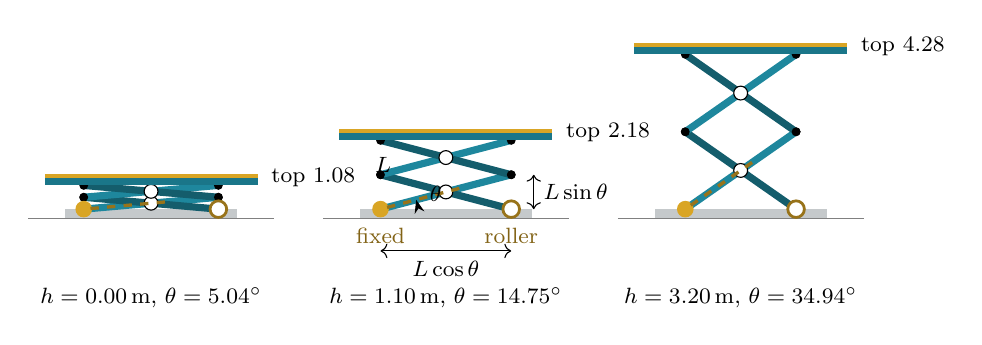
\begin{tikzpicture}[x=0.52cm,y=0.52cm,font=\footnotesize]
\begin{scope}[shift={(0.00,0)}]
\draw[gray] (-3.0,0) -- (3.0,0);
\fill[smsteel!40] (-2.1,0) rectangle (2.1,0.220);
\draw[line width=2.6pt,smcyan!80!black] (-1.644,0.220) -- (1.644,0.510);
\draw[line width=2.6pt,smcyan!55!black] (1.644,0.220) -- (-1.644,0.510);
\fill[white,draw=black] (0,0.365) circle (2.5pt);
\fill[black] (-1.644,0.220) circle (1.6pt);
\fill[black] (-1.644,0.510) circle (1.6pt);
\fill[black] (1.644,0.220) circle (1.6pt);
\fill[black] (1.644,0.510) circle (1.6pt);
\draw[line width=2.6pt,smcyan!80!black] (-1.644,0.510) -- (1.644,0.800);
\draw[line width=2.6pt,smcyan!55!black] (1.644,0.510) -- (-1.644,0.800);
\fill[white,draw=black] (0,0.655) circle (2.5pt);
\fill[black] (-1.644,0.510) circle (1.6pt);
\fill[black] (-1.644,0.800) circle (1.6pt);
\fill[black] (1.644,0.510) circle (1.6pt);
\fill[black] (1.644,0.800) circle (1.6pt);
\fill[smamber] (-1.644,0.220) circle (3pt);
\draw[smamber!70!black,fill=white,line width=1pt] (1.644,0.220) circle (3pt);
\draw[dashed,line width=1.2pt,smamber!70!black] (-1.479,0.234) -- (0.394,0.400);
\fill[smcyan!70!black] (-2.6,0.800) rectangle (2.6,0.980);
\fill[smamber] (-2.6,0.980) rectangle (2.6,1.080);
\node[below] at (0,-1.45) {$h=0.00$\,m,\ $\theta=5.04^\circ$};
\node[right] at (2.7,1.000) {top $1.08$};
\end{scope}
\begin{scope}[shift={(7.20,0)}]
\draw[gray] (-3.0,0) -- (3.0,0);
\fill[smsteel!40] (-2.1,0) rectangle (2.1,0.220);
\draw[line width=2.6pt,smcyan!80!black] (-1.596,0.220) -- (1.596,1.060);
\draw[line width=2.6pt,smcyan!55!black] (1.596,0.220) -- (-1.596,1.060);
\fill[white,draw=black] (0,0.640) circle (2.5pt);
\fill[black] (-1.596,0.220) circle (1.6pt);
\fill[black] (-1.596,1.060) circle (1.6pt);
\fill[black] (1.596,0.220) circle (1.6pt);
\fill[black] (1.596,1.060) circle (1.6pt);
\draw[line width=2.6pt,smcyan!80!black] (-1.596,1.060) -- (1.596,1.900);
\draw[line width=2.6pt,smcyan!55!black] (1.596,1.060) -- (-1.596,1.900);
\fill[white,draw=black] (0,1.480) circle (2.5pt);
\fill[black] (-1.596,1.060) circle (1.6pt);
\fill[black] (-1.596,1.900) circle (1.6pt);
\fill[black] (1.596,1.060) circle (1.6pt);
\fill[black] (1.596,1.900) circle (1.6pt);
\fill[smamber] (-1.596,0.220) circle (3pt);
\draw[smamber!70!black,fill=white,line width=1pt] (1.596,0.220) circle (3pt);
\draw[dashed,line width=1.2pt,smamber!70!black] (-1.436,0.262) -- (0.383,0.741);
\fill[smcyan!70!black] (-2.6,1.900) rectangle (2.6,2.080);
\fill[smamber] (-2.6,2.080) rectangle (2.6,2.180);
\node[below] at (0,-1.45) {$h=1.10$\,m,\ $\theta=14.75^\circ$};
\node[right] at (2.7,2.100) {top $2.18$};
\draw[-{Stealth}] (-0.696,0.220) arc (0:14.75:0.9);
\node at (-0.246,0.600) {$\theta$};
\node[above left] at (-1.098,0.875) {$L$};
\draw[<->] (2.146,0.220) -- (2.146,1.060) node[midway,right] {$L\sin\theta$};
\draw[<->] (-1.596,-0.80) -- (1.596,-0.80) node[midway,below] {$L\cos\theta$};
\node[smamber!60!black,below] at (-1.596,0.000) {fixed};
\node[smamber!60!black,below] at (1.596,0.000) {roller};
\end{scope}
\begin{scope}[shift={(14.40,0)}]
\draw[gray] (-3.0,0) -- (3.0,0);
\fill[smsteel!40] (-2.1,0) rectangle (2.1,0.220);
\draw[line width=2.6pt,smcyan!80!black] (-1.353,0.220) -- (1.353,2.110);
\draw[line width=2.6pt,smcyan!55!black] (1.353,0.220) -- (-1.353,2.110);
\fill[white,draw=black] (0,1.165) circle (2.5pt);
\fill[black] (-1.353,0.220) circle (1.6pt);
\fill[black] (-1.353,2.110) circle (1.6pt);
\fill[black] (1.353,0.220) circle (1.6pt);
\fill[black] (1.353,2.110) circle (1.6pt);
\draw[line width=2.6pt,smcyan!80!black] (-1.353,2.110) -- (1.353,4.000);
\draw[line width=2.6pt,smcyan!55!black] (1.353,2.110) -- (-1.353,4.000);
\fill[white,draw=black] (0,3.055) circle (2.5pt);
\fill[black] (-1.353,2.110) circle (1.6pt);
\fill[black] (-1.353,4.000) circle (1.6pt);
\fill[black] (1.353,2.110) circle (1.6pt);
\fill[black] (1.353,4.000) circle (1.6pt);
\fill[smamber] (-1.353,0.220) circle (3pt);
\draw[smamber!70!black,fill=white,line width=1pt] (1.353,0.220) circle (3pt);
\draw[dashed,line width=1.2pt,smamber!70!black] (-1.217,0.315) -- (0.325,1.392);
\fill[smcyan!70!black] (-2.6,4.000) rectangle (2.6,4.180);
\fill[smamber] (-2.6,4.180) rectangle (2.6,4.280);
\node[below] at (0,-1.45) {$h=3.20$\,m,\ $\theta=34.94^\circ$};
\node[right] at (2.7,4.200) {top $4.28$};
\end{scope}
\end{tikzpicture}
}\\[3pt]
\begin{subfigure}{0.49\textwidth}\shot{\linewidth}{images/lift/lift_mechanism.jpg}\caption{The mechanism at $h=1.10$ (rendered)}\end{subfigure}\hfill
\begin{subfigure}{0.49\textwidth}\shot{\linewidth}{images/lift/lift_scissor.jpg}\caption{The lift raised to $h=2.0$ (rendered)}\end{subfigure}
\caption{Side view drawn to scale at three heights ($z$ horizontal, $y$ vertical). Cyan = the two arms of each X, white dot = centre pin, amber disc = fixed pivot, open circle =
sliding roller, dashed line = hydraulic ram, blue/amber slab = platform beam and runway pad. Below: the same lift as rendered by the program.}\label{fig:scissor}
\end{figure}
\textbf{Step-by-step.}
\begin{enumerate}[leftmargin=*,label=\textbf{\arabic*.}]
\item \emph{One arm.} An arm of length $L=3.30$ at angle $\theta$ gains height $L\sin\theta$ and covers a horizontal span $L\cos\theta$ between its pivots.
\item \emph{Two stages.} The upper X stands on the lower X, so the platform underside is at $y=0.22+2L\sin\theta$ ($0.22$ is the top of the base frame).
\item \emph{From height to angle.} The program is given a lift height $h$ (\fn{gLiftHeight}; keys \fn{P}, \fn{[} \fn{]}, or the service). At rest the platform is
already $0.58$ above the frame (\fn{LIFT\_REST\_H}), so $2L\sin\theta=0.58+h$. Solving for the angle:
\begin{equation}\theta=\arcsin\!\Big(\frac{0.58+h}{2L}\Big),\;L=3.30,\qquad \text{\fn{liftTopY}}(h)=0.22+2L\sin\theta+0.18+0.10=1.08+h .\label{eq:scissor}\end{equation}
\item \emph{The surface the tyres stand on.} Beam $0.18$ and runway pad $0.10$ are added, giving $y_{\text{top}}=1.08+h$. The vehicle matrix uses exactly this
number, so raising the lift raises the car with no other change.
\item \emph{The roller slides.} The span $L\cos\theta$ shrinks as the arms stand up, so the roller moves toward the fixed pivot: from $3.287$ at $h=0$ to $2.705$ at
$h=3.2$, i.e.\ $0.58$ m of travel (it is drawn at $(x,\,y_{\text{bottom}}+0.02,\,+\text{halfSpan})$, halfSpan $=L\cos\theta/2$).
\end{enumerate}
\begin{table}[!htbp]\centering\scriptsize
\caption{Worked values of Eq.~\eqref{eq:scissor} (all computed from $L=3.30$, base $0.22$). $h=1.10$ is the service height, $h=3.20$ the \fn{P} key target.}\label{tab:liftvalues}
\begin{tabular}{@{}rrrrrrr@{}}\toprule
$h$ (m) & $\sin\theta$ & $\theta$ & $L\sin\theta$ (stage rise) & $L\cos\theta$ (span) & $2L\sin\theta$ & $y_{\text{top}}=1.08+h$\\\midrule
0.00 & 0.0879 & $5.04^\circ$ & 0.290 & 3.287 & 0.58 & 1.08\\
0.50 & 0.1636 & $9.42^\circ$ & 0.540 & 3.256 & 1.08 & 1.58\\
1.10 & 0.2545 & $14.75^\circ$ & 0.840 & 3.191 & 1.68 & 2.18\\
2.00 & 0.3909 & $23.01^\circ$ & 1.290 & 3.037 & 2.58 & 3.08\\
3.20 & 0.5727 & $34.94^\circ$ & 1.890 & 2.705 & 3.78 & 4.28\\\bottomrule
\end{tabular}
\end{table}
\textbf{How the code draws one stack.} For each stage $s=0,1$ the bottom pivots are at $y_b=0.22+s\,L\sin\theta$ and the arms cross at $y_{\text{mid}}=y_b+L\sin\theta/2$.
Arm A is a cube $S(0.20,0.32,3.30)$ rotated $R_x(-\theta)$ at $(x-0.12,\,y_{\text{mid}},\,0)$; arm B is the \emph{same cube} rotated $R_x(+\theta)$ at $(x+0.12,\,y_{\text{mid}},\,0)$ --- the mirror
rotation is what makes the X, and the $0.24$ offset in $x$ stops the two arms sharing a plane. Four pivot pins, bearing collars, a centre pin, the yellow roller and the
connecting plates are placed at $z=\pm\text{halfSpan}$ and $y=y_b,\,y_b+L\sin\theta$. \textbf{The ram} is a chrome rod ($0.84L$ long) inside a dark barrel ($0.52L$) lying along arm A: a part
a fraction $f$ of the way up the arm is at $P(f)=P_0+f\,L\,(0,\sin\theta,\cos\theta)$, and because a cylinder's own axis is $+y$ it is turned by $R_x(90^\circ-\theta)$. The ram is
positioned relative to arm A, so it tilts with the arm; it is not a separate extension simulation.\\
\textbf{Motion and safety.} \fn{gLiftHeight} moves at \fn{kLiftSpeed}$=0.55$ m/s, so the automatic LIFT\_UP ($0\to1.10$) takes $1.10/0.55=2.0$ s (state time in Fig.~\ref{fig:fsm}); a manual move
is refused by \fn{liftPositionSafe()} if the robot arm would hit the raised platform or vehicle, or if $h$ leaves $[0,3.80]$.
\begin{figure}[!htbp]\centering
\begin{subfigure}{0.32\textwidth}\shot{\linewidth}{images/lift/build_01.jpg}\caption{1: base rails, tracks, anchors}\end{subfigure}\hfill
\begin{subfigure}{0.32\textwidth}\shot{\linewidth}{images/lift/build_02.jpg}\caption{2: left scissor stack + ram}\end{subfigure}\hfill
\begin{subfigure}{0.32\textwidth}\shot{\linewidth}{images/lift/build_03.jpg}\caption{3: right scissor stack + ram}\end{subfigure}\\[2pt]
\begin{subfigure}{0.32\textwidth}\shot{\linewidth}{images/lift/build_04.jpg}\caption{4: platform cross beams}\end{subfigure}\hfill
\begin{subfigure}{0.32\textwidth}\shot{\linewidth}{images/lift/build_05.jpg}\caption{5: left runway}\end{subfigure}\hfill
\begin{subfigure}{0.32\textwidth}\shot{\linewidth}{images/lift/build_06.jpg}\caption{6: right runway (complete)}\end{subfigure}
\caption{Actual construction order of \fn{drawHydraulicLift()} at $h=1.10$ (key \fn{3}, then \fn{N}/\fn{B}); amber = part added in that step. Step values: base rail $S(0.66,0.22,3.90)$, cross members $S(2.60,0.18,0.34)$ at $z=\pm1.80$, platform beams $S(2.70,0.16,0.34)$ at $z=\pm1.55$, runway beam $S(0.88,0.18,5.20)$, pad $S(1.00,0.10,5.20)$.}\label{fig:lift-build}
\end{figure}
\begin{figure}[!htbp]\centering
\begin{subfigure}{0.32\textwidth}\shot{\linewidth}{images/orthographic/lift_right_lab.png}\caption{Right-Side View, parts A--G}\end{subfigure}\hfill
\begin{subfigure}{0.32\textwidth}\shot{\linewidth}{images/orthographic/lift_front_dim.png}\caption{Front View}\end{subfigure}\hfill
\begin{subfigure}{0.32\textwidth}\shot{\linewidth}{images/orthographic/lift_top_dim.png}\caption{Top View}\end{subfigure}
\caption{Hydraulic lift three-view at $h=1.10$\,m. A base rail, B scissor arms, C centre pin, D ram, E platform beam, F runway pad, G anchor plate.}\label{fig:lift}
\end{figure}
\viva{Scissor lift}{\fn{SceneObjects.cpp}, \fn{Main.cpp}}{\fn{scissorAngle()}, \fn{drawScissorStack()}, \fn{drawHydraulicLift()}, \fn{liftTopY()}}
{\fn{LIFT\_ARM\_LEN}=3.30, \fn{LIFT\_REST\_H}=0.58, \fn{LIFT\_BASE\_TOP}=0.22, \fn{LIFT\_TRACK}=0.98, \fn{gLiftHeight} (0--3.80), \fn{kLiftSpeed}=0.55\,m/s, \fn{kServiceLiftTarget}=1.10}
{raising \fn{gLiftHeight} increases $\theta$ (Table~\ref{tab:liftvalues}), opens the X and carries the vehicle; larger \fn{kLiftSpeed} raises faster; longer \fn{LIFT\_ARM\_LEN} gives a smaller $\theta$ for the same height; larger \fn{LIFT\_REST\_H} raises the lowest position.}
{Eq.~\eqref{eq:scissor}; Figs.~\ref{fig:scissor}, \ref{fig:lift-build}, \ref{fig:lift}}

% ---------------------------------------------------------------- robot
\subsection{Robotic arm: construction sequence and calculation}
The arm is built bottom-up; every step adds parts in the frame of its parent, so one product of matrices places each part:
\begin{equation}\begin{gathered}
M_{\text{turn}}=T(-4.6,0,-2.2)R_y(\gamma),\quad M_1=M_{\text{turn}}T(0,1.05,0)R_z(\theta_1),\quad M_2=M_1T(0,4.5,0)R_z(\theta_2),\\
M_{\text{wrist}}=M_2T(0,4.0,0)R_z(\omega)R_y(\rho),\qquad M_{\text{tool}}=M_{\text{wrist}}T(0,-0.16,0).
\end{gathered}\label{eq:robotchain}\end{equation}
Each link is \fn{place((0,L/2,0),(w,L,d))} in its joint frame, so its bottom sits on the joint and the joint is the pivot.
\begin{figure}[!htbp]\centering
\begin{subfigure}{0.24\textwidth}\shot{\linewidth}{images/robot/build_01.jpg}\caption{1: base plate, 4 bolts}\end{subfigure}\hfill
\begin{subfigure}{0.24\textwidth}\shot{\linewidth}{images/robot/build_02.jpg}\caption{2: pedestal + status band}\end{subfigure}\hfill
\begin{subfigure}{0.24\textwidth}\shot{\linewidth}{images/robot/build_03.jpg}\caption{3: turntable disc}\end{subfigure}\hfill
\begin{subfigure}{0.24\textwidth}\shot{\linewidth}{images/robot/build_04.jpg}\caption{4: shoulder yoke}\end{subfigure}\\[2pt]
\begin{subfigure}{0.24\textwidth}\shot{\linewidth}{images/robot/build_05.jpg}\caption{5: shoulder joint}\end{subfigure}\hfill
\begin{subfigure}{0.24\textwidth}\shot{\linewidth}{images/robot/build_06.jpg}\caption{6: lower arm $L_1$}\end{subfigure}\hfill
\begin{subfigure}{0.24\textwidth}\shot{\linewidth}{images/robot/build_07.jpg}\caption{7: elbow joint}\end{subfigure}\hfill
\begin{subfigure}{0.24\textwidth}\shot{\linewidth}{images/robot/build_08.jpg}\caption{8: forearm $L_2$}\end{subfigure}\\[2pt]
\begin{subfigure}{0.24\textwidth}\shot{\linewidth}{images/robot/build_09.jpg}\caption{9: wrist + coupler}\end{subfigure}\hfill
\begin{subfigure}{0.24\textwidth}\shot{\linewidth}{images/robot/build_10.jpg}\caption{10: scanner tool head}\end{subfigure}\hfill
\begin{subfigure}{0.24\textwidth}\shot{\linewidth}{images/robot/robot_home.jpg}\caption{Result in the scene (HOME pose)}\end{subfigure}\hfill
\begin{subfigure}{0.24\textwidth}\centering\resizebox{\linewidth}{!}{% Planar chain in the turntable frame for pose (gamma, th1, th2, omega) = (0, -30, -60, 90), scanner fitted.
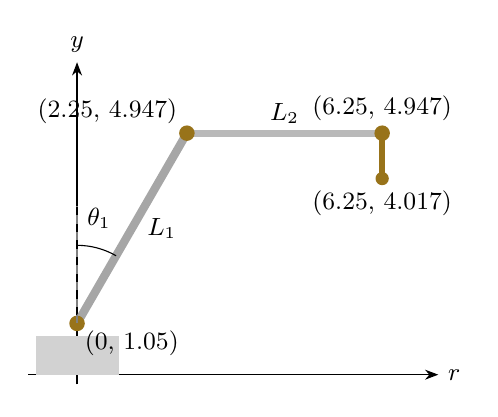
\begin{tikzpicture}[x=0.62cm, y=0.62cm, font=\small]
  \draw[-{Stealth}] (-1.0,0) -- (7.4,0) node[right]{$r$};
  \draw[-{Stealth}] (0,-0.2) -- (0,6.4) node[above]{$y$};
  \fill[gray!35] (-0.85,0) rectangle (0.85,0.8);
  \coordinate (S) at (0,1.05);
  \coordinate (E) at (2.25,4.947);
  \coordinate (W) at (6.25,4.947);
  \coordinate (T) at (6.25,4.017);
  \draw[line width=3pt, gray!70] (S) -- (E);
  \draw[line width=2.6pt, gray!55] (E) -- (W);
  \draw[line width=2pt, smamber!70!black] (W) -- (T);
  \foreach \p in {S,E,W} \fill[smamber!70!black] (\p) circle (2.8pt);
  \fill[smamber!70!black] (T) circle (2.4pt);
  \node[below right=-1pt] at (S) {$(0,\,1.05)$};
  \node[above left] at (E) {$(2.25,\,4.947)$};
  \node[above] at ($(W)+(0,0.05)$) {$(6.25,\,4.947)$};
  \node[below] at ($(T)+(0,-0.05)$) {$(6.25,\,4.017)$};
  \draw[dashed, gray] (S) -- ++(0,2.4);
  \draw ($(S)+(0,1.6)$) arc (90:60:1.6);
  \node at ($(S)+(0.45,2.15)$) {$\theta_1$};
  \node[above] at ($(E)!0.5!(W)$) {$L_2$};
  \node[right=2pt] at ($(S)!0.5!(E)$) {$L_1$};
\end{tikzpicture}
}\caption{Kinematic chain (see caption)}\end{subfigure}
\caption{Actual construction order of \fn{drawRobotArm()} (key \fn{4}, then \fn{N}/\fn{B}) at $(\gamma,\theta_1,\theta_2,\omega)=(0,-30^\circ,-60^\circ,90^\circ)$; steps 1--5 are zoomed on the pedestal. (l) Kinematic chain of this pose: $L_1=4.5$, $L_2=4.0$; $\theta_1{+}\theta_2=-90^\circ$ makes the forearm horizontal and $\theta_1{+}\theta_2{+}\omega=0$ makes the tool hang vertically.}\label{fig:robot-build}
\end{figure}
\textbf{Joint ranges and rates} (\fn{Main.cpp}): base yaw \fn{gRobotBaseYaw} $\pm180^\circ$ (\fn{T/G}, $45^\circ$/s); shoulder \fn{gJoint1Angle} $-110^\circ\ldots55^\circ$ (\fn{U/J}, $35^\circ$/s);
elbow \fn{gJoint2Angle} $-150^\circ\ldots120^\circ$ (\fn{I/K}, $35^\circ$/s); wrist pitch \fn{gWristPitch} $\pm270^\circ$ (\fn{Y/H}, $55^\circ$/s); wrist roll \fn{gWristRoll} $\pm180^\circ$ ($\leftarrow/\rightarrow$, $55^\circ$/s);
tool \fn{gRobotTool} 0..3 (\fn{F1}--\fn{F4}); HOME $=(60,-44,-30,74,0)$.
\textbf{Worked calculation.} Forward kinematics in the turntable plane (identical to \fn{robotSafetyPoints()}):
\begin{equation}\begin{gathered}\vect e=(-L_1\sin\theta_1,\;1.05+L_1\cos\theta_1),\qquad
\vect w=\vect e+\big(-L_2\sin(\theta_1{+}\theta_2),\;L_2\cos(\theta_1{+}\theta_2)\big),\\
\vect t=\vect w+\ell\big(\sin\Sigma,\,-\cos\Sigma\big),\qquad\Sigma=\theta_1{+}\theta_2{+}\omega .\end{gathered}\label{eq:fk}\end{equation}
For the pose of Fig.~\ref{fig:robot-build}: $\vect e=(4.5\sin30^\circ,\,1.05+4.5\cos30^\circ)=(2.250,\,4.947)$;
$\theta_1{+}\theta_2=-90^\circ\Rightarrow\vect w=(2.25+4.0,\;4.947+0)=(6.250,\,4.947)$; $\Sigma=0\Rightarrow$ scanner lens
($\ell=0.93$) at $(6.250,\,4.017)$. Link centres (steps 6 and 8): lower arm $(1.125,\,2.999)$, forearm $(4.250,\,4.947)$; the
two cable bands of step 6 are at $y=1.05+1.44\cos30^\circ=2.297$ and $1.05+3.06\cos30^\circ=3.700$. Poses were solved offline
with two-link inverse kinematics, $D=\frac{x^2+y^2-L_1^2-L_2^2}{2L_1L_2}$, $\theta_2=\operatorname{atan2}(\pm\sqrt{1-D^2},D)$; recomputing
\fn{POSE\_LUG\_1} from its wrist point gives $\theta_1=5.05^\circ$, $\theta_2=-139.01^\circ$ exactly (reachable annulus
$0.5\le r\le8.5$).
\begin{figure}[!htbp]\centering
\begin{subfigure}{0.455\textwidth}\shot{\linewidth}{images/orthographic/robot_front_dim.png}\caption{Front View}\end{subfigure}\hfill
\begin{subfigure}{0.455\textwidth}\shot{\linewidth}{images/orthographic/robot_vars.png}\caption{Joint variables and rotation axes}\end{subfigure}\\[2pt]
\begin{subfigure}{0.455\textwidth}\shot{\linewidth}{images/orthographic/robot_top_dim.png}\caption{Top View}\end{subfigure}\hfill
\begin{subfigure}{0.455\textwidth}\shot{\linewidth}{images/orthographic/robot_right_dim.png}\caption{Right-Side View}\end{subfigure}
\caption{Robot three-view at $(\gamma,\theta_1,\theta_2,\omega)=(0,-30^\circ,-60^\circ,90^\circ)$; (b) labels every joint with its \fn{Main.cpp} variable and rotation axis (arrows show the positive rotation).}\label{fig:robot}
\end{figure}
\viva{Robot arm (5-DOF)}{\fn{SceneObjects.cpp} (geometry), \fn{Main.cpp} (angles, poses, limits)}{\fn{drawRobotArm()}, \fn{moveRobotTowardPose()}, \fn{processMovement()}}
{\fn{ARM\_X,ARM\_Z}=$(-4.6,-2.2)$, \fn{ARM\_SHOULDER\_Y}=1.05, \fn{ARM\_LOWER\_LEN}=4.50, \fn{ARM\_UPPER\_LEN}=4.00, joint ranges above, \fn{POSE\_HOME}}
{increasing \fn{gJoint1Angle} swings the whole chain toward $-x$ ($R_z$ turns $+y$ toward $-x$); every child (elbow, wrist, tool, spotlight) follows because each frame is multiplied onto its parent; changing a link length moves all frames above it.}
{Eqs.~\eqref{eq:robotchain}, \eqref{eq:fk}; Figs.~\ref{fig:robot-build}, \ref{fig:robot}}

% ---------------------------------------------------------------- tools
\subsection{Tool station (the table) and the tool exchange: how it works}\label{sec:station}
\textbf{What it is.} The tool station is an open steel table beside the robot, built in the frame $T(-7.9,0,-1.85)$ (that is the robot base $(-4.6,-2.2)$ moved by
$(-3.30,+0.35)$). It has \textbf{four docks}, one per quick-change tool, in a $2\times2$ grid so the wrist can drop straight onto one dock without touching its neighbour. A dock is a short
chrome connector post on a dark pedestal; a tool stands on it exactly as it will later sit on the robot's coupler. The gripper also picks up a loose \emph{sponge} from the middle of the table (Fig.~\ref{fig:station}).
\begin{figure}[!htbp]\centering
\begin{minipage}[c]{0.40\textwidth}\centering\resizebox{\linewidth}{!}{% tool station, top view (x right, z down), dimensions from drawRobotToolStation()
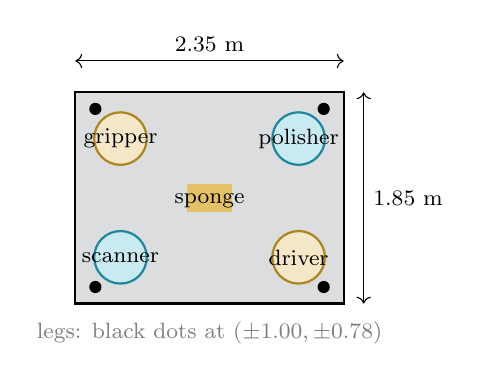
\begin{tikzpicture}[x=1.45cm,y=1.45cm,font=\footnotesize]
\fill[smsteel!25] (-1.175,-0.925) rectangle (1.175,0.925);
\draw[thick] (-1.175,-0.925) rectangle (1.175,0.925);
\foreach \sx in {-1,1} \foreach \sz in {-1,1} \fill[black] (\sx*1.0,\sz*0.78) circle (2.2pt);
\draw[fill=smcyan!25,draw=smcyan!80!black,thick] (-0.78,-0.52) circle (0.23);
\node at (-0.78,-0.52) {scanner};
\draw[fill=smamber!25,draw=smamber!80!black,thick] (0.78,-0.52) circle (0.23);
\node at (0.78,-0.52) {driver};
\draw[fill=smamber!25,draw=smamber!80!black,thick] (-0.78,0.52) circle (0.23);
\node at (-0.78,0.52) {gripper};
\draw[fill=smcyan!25,draw=smcyan!80!black,thick] (0.78,0.52) circle (0.23);
\node at (0.78,0.52) {polisher};
\fill[smamber!70] (-0.2,-0.12) rectangle (0.2,0.12); \node[below] at (0,0.12) {sponge};
\draw[<->] (-1.175,1.2) -- (1.175,1.2) node[midway,above] {2.35 m};
\draw[<->] (1.35,-0.925) -- (1.35,0.925) node[midway,right] {1.85 m};
\node[gray] at (0,-1.18) {legs: black dots at $(\pm1.00,\pm0.78)$};
\end{tikzpicture}
}\end{minipage}\hfill
\begin{minipage}[c]{0.57\textwidth}\centering\shot{\linewidth}{images/tools/tool_rack.jpg}\end{minipage}
\caption{Tool station in plan (left, to scale, table-local $x$ right and $z$ down) and as rendered with all four tools docked (right). Dock positions $(\pm0.78,\,0.975,\,\pm0.52)$.}\label{fig:station}
\end{figure}
\textbf{Numbers (\fn{drawRobotToolStation}).} Tabletop $S(2.35,0.11,1.85)$ at $y=0.78$ (top face $0.835$); under-frame $S(2.20,0.06,1.70)$ at $y=0.70$; four legs $S(0.11,0.74,0.11)$ at $(\pm1.00,0.37,\pm0.78)$;
two low stretchers at $y=0.17$. Dock pedestal $S(0.46,0.05,0.46)$ at $y=0.865$, ring $y=0.905$, connector post at $y=0.945$ whose top is the dock height $0.975$ (\fn{kToolDockTopY}).
\textbf{How it behaves.} The station is told which tool is on the arm (\fn{selectedTool}). That dock is empty, so its pedestal ring and the small status lamp in the tabletop \emph{glow cyan};
the other three docks show their tool standing on the connector, lifted by its own drop so that its lowest point just touches it:
\begin{equation}\begin{gathered}y_{\text{tool}}=0.975+\text{\fn{toolBottomDrop}}\cdot k_{\text{rack}}\\
0.975+0.770=1.745\;(\text{scanner}),\quad 1.965\;(\text{driver}),\quad 1.845\;(\text{gripper}),\quad 1.747\;(\text{polisher}).\end{gathered}\label{eq:dock}\end{equation}
The world position of a dock is $T(-7.9,0,-1.85)$ applied to its local position: $(-8.68,\,0.975,\,-2.37)$ scanner, $(-7.12,-2.37)$ driver, $(-8.68,-1.33)$ gripper, $(-7.12,-1.33)$ polisher.
\textbf{The exchange, step by step} (\fn{runToolChange()}; every step is slow and visible): (0) swing clear of the vehicle and over the rack; (1) line up $0.70$ above the dock the current tool came from; (2) descend slowly onto it;
(3) pause, then \emph{release} --- the tool stays on the dock and the arm becomes a bare coupler; (4) lift clear; (5) hold $0.55$ s so a bare coupler and both tools are visible together; (6) travel above the next dock;
(7) descend; (8) pause, then \emph{latch} --- the new tool becomes part of the arm; (9) lift it off the dock (Fig.~\ref{fig:toolchange}).
\textbf{Dock check by forward kinematics.} For \fn{POSE\_DOCK\_SEAT[0]} $=(177.61^\circ,-23.40^\circ,-121.56^\circ,144.96^\circ)$:
$\Sigma=-23.40-121.56+144.96=0^\circ$ (tool vertical); $\vect e=(1.787,5.180)$, $\vect w=(4.084,1.905)$,
$\vect t=(4.084,\,0.975)$; yaw $177.61^\circ$ gives world $x=-4.6+4.084\cos177.61^\circ=-8.680$ and
$z=-2.2-4.084\sin177.61^\circ=-2.370$ --- exactly the dock position above; the other three seat poses reproduce their docks to within \SI{3}{mm}.
\begin{figure}[!htbp]\centering
\begin{subfigure}{0.245\textwidth}\shot{\linewidth}{images/orthographic/tool_scanner_front_dim.png}\caption{Scanner}\end{subfigure}\hfill
\begin{subfigure}{0.245\textwidth}\shot{\linewidth}{images/orthographic/tool_driver_front_dim.png}\caption{Impact driver}\end{subfigure}\hfill
\begin{subfigure}{0.245\textwidth}\shot{\linewidth}{images/orthographic/tool_gripper_front_dim.png}\caption{Gripper}\end{subfigure}\hfill
\begin{subfigure}{0.245\textwidth}\shot{\linewidth}{images/orthographic/tool_polisher_front_dim.png}\caption{Polisher}\end{subfigure}
\caption{The four tool heads (front orthographic views, ``drop'' = \fn{toolBottomDrop()}).}\label{fig:tools}
\end{figure}
Tool numbers: scanner housing $0.62{\times}0.34{\times}0.76$ with a cyan lens at $y=-0.74$; the driver socket spins
$R_y(\text{driverAngle})$ at \SI{980}{\degree/s} and its tip is $1.15$ from the wrist; gripper fingers sit at $x=\pm(0.18+0.16\,o)$ with
opening $o\in[0,1]$ and tilt $\mp8^\circ(1-0.35\,o)$; the polisher pad \O\,0.58 spins at \SI{620}{\degree/s}. A held sponge is drawn in
$M_{\text{tool}}T(0,-0.91,0)$: parenting is the attachment.
\begin{figure}[!htbp]\centering
\begin{subfigure}{0.32\textwidth}\shot{\linewidth}{images/service/tool_exchange_a_release.jpg}\caption{$t=74.6$ s: scanner seated}\end{subfigure}\hfill
\begin{subfigure}{0.32\textwidth}\shot{\linewidth}{images/service/tool_exchange_b_bare.jpg}\caption{$t=77.5$ s: bare coupler}\end{subfigure}\hfill
\begin{subfigure}{0.32\textwidth}\shot{\linewidth}{images/service/tool_exchange_c_grasp.jpg}\caption{$t=80.5$ s: gripper takes sponge}\end{subfigure}
\caption{Visible tool exchange during the GET\_SPONGE state.}\label{fig:toolchange}
\end{figure}
\viva{Tool station (table)}{\fn{SceneObjects.cpp}, \fn{Main.cpp}}{\fn{drawRobotToolStation()}, \fn{toolDockPosition()}, \fn{runToolChange()}}
{table $2.35{\times}1.85$, top $0.835$; \fn{kToolDockTopY}=0.975; docks $(\pm0.78,\pm0.52)$; frame $T(-7.9,0,-1.85)$; \fn{POSE\_DOCK\_HOVER/SEAT}; speed scales 0.24--1.25}
{moving \fn{kToolDockTopY} lifts all docks (the seat poses must then be re-solved); a larger speed scale makes the exchange faster; a different drop value changes how a tool sits on the connector; changing the dock grid moves where the arm descends.}
{Eq.~\eqref{eq:dock}; Figs.~\ref{fig:station}, \ref{fig:tools}, \ref{fig:toolchange}}

% ---------------------------------------------------------------- door ramp turntable
\subsection{Roller garage door: how it works}\label{sec:door}
\textbf{What it is.} A roller shutter: five flat panels (each $13.0$ m wide and $0.98$ m high, together the $4.9$ m opening) held in two C-section guide rails. A motor turns a shaft
at the top; the panels slide up the rails and then \emph{wind round a drum} above the opening, just like a real shutter. The only animated number is the \textbf{door offset} $d$ (\fn{gDoorOffset}, metres):
$d=0$ closed, $d=4.9$ open. Keys \fn{O}, \fn{Z/X/C} and the state machine only change the target \fn{gDoorTarget}; \fn{moveToward()} then moves $d$ at \fn{kDoorSpeed}$=0.8$ m/s, so a full opening takes $4.9/0.8=6.125$ s
(the DOOR\_OPEN\_IN and DOOR\_OPEN states in Fig.~\ref{fig:fsm}). While it moves, an amber warning beacon pulses.
\textbf{Step-by-step (what happens to panel $i=0..4$, bottom to top).}
\begin{enumerate}[leftmargin=*,label=\textbf{\arabic*.}]
\item \emph{Straight travel.} If it only slid up, the centre of panel $i$ would be at $\text{travel}_i=0.98\,(0.5+i)+d$.
\item \emph{How far past the top?} $\text{over}=\text{travel}_i-4.9$. While $\text{over}\le0$ the panel is flat in the rails: its matrix is just $T(0,\text{travel}_i,z_d)$.
\item \emph{Winding.} When $\text{over}>0$ the extra travel is turned into an angle round the drum shaft (arc length divided by radius): $\alpha=\text{over}/R$ with drum radius $R=0.52$.
One panel ($0.98$ long) therefore uses $0.98/0.52=1.88$ rad $\approx108^\circ$ of drum, and the five panels wrap about one and a half turns.
\item \emph{Layers.} Each full turn lies on top of the last, so the radius grows by one panel thickness ($0.095$) per revolution: $r=R+0.095\,\alpha/360^\circ$. The angle is capped at $560^\circ$ (drum full).
\item \emph{Placing the panel.} Rotate about the shaft, step out to the radius, then lay the panel's length along the circumference (the shaft lies along $x$, so the rotations are about $x$):
\end{enumerate}
\begin{equation}\alpha=\frac{\text{over}}{R},\qquad r=R+0.095\frac{\alpha}{2\pi},\qquad M_{\text{panel}}=T(0,5.85,z_d)\,R_x(\alpha)\,T(0,-r,0)\,R_x(90^\circ),\label{eq:door}\end{equation}
where $5.85=\text{DOOR\_H}+0.95$ is the height of the drum centre and $z_d=12.88$ the door plane.
\begin{table}[!htbp]\centering\scriptsize
\caption{Door state for five offsets $d$ (computed from Eq.~\eqref{eq:door}): ``flat'' = still in the rails, otherwise the winding angle $\alpha$ of that panel.}\label{tab:doorvalues}
\begin{tabular}{@{}rccccc@{}}\toprule
$d$ (m) & panel 0 & panel 1 & panel 2 & panel 3 & panel 4\\\midrule
0.00 & flat & flat & flat & flat & flat\\
1.50 & flat & flat & flat & $3.3^\circ$ & $111.3^\circ$\\
2.45 & flat & flat & flat & $108.0^\circ$ ($r=0.548$) & $216.0^\circ$ ($r=0.577$)\\
3.50 & flat & $7.7^\circ$ & $115.7^\circ$ & $223.7^\circ$ & $331.7^\circ$\\
4.90 & $54.0^\circ$ & $162.0^\circ$ & $270.0^\circ$ & $377.9^\circ$ & $485.9^\circ$ ($r=0.648$)\\\bottomrule
\end{tabular}
\end{table}
\begin{figure}[!htbp]\centering
\begin{subfigure}{0.32\textwidth}\shot{\linewidth}{images/objects/door_closed.jpg}\caption{$d=0$: closed}\end{subfigure}\hfill
\begin{subfigure}{0.32\textwidth}\shot{\linewidth}{images/objects/door_half.jpg}\caption{$d=2.45$: panels 3, 4 winding}\end{subfigure}\hfill
\begin{subfigure}{0.32\textwidth}\shot{\linewidth}{images/objects/door_open.jpg}\caption{$d=4.9$: open, rolled on drum}\end{subfigure}\\[2pt]
\begin{minipage}[c]{0.55\textwidth}\centering\resizebox{\linewidth}{!}{% Roller-shutter geometry (side view, y up, z right): panel travel, drum radius, winding angle.
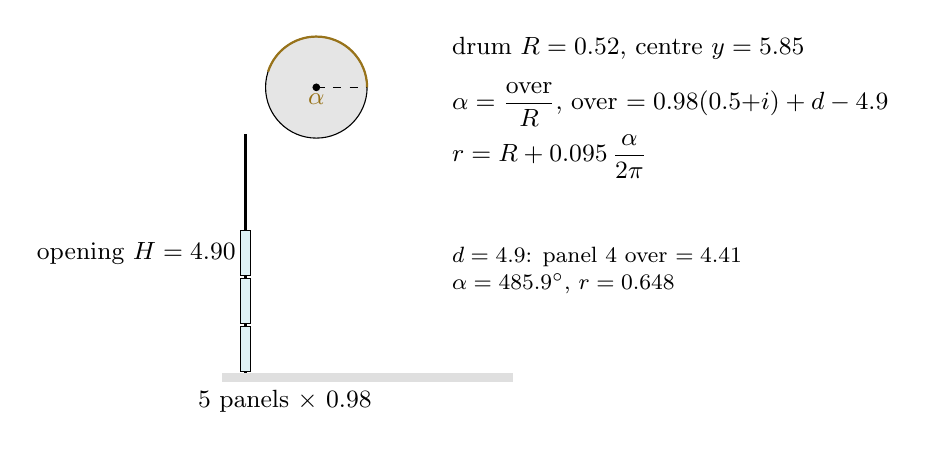
\begin{tikzpicture}[x=1.0cm, y=1.0cm, font=\small]
  % opening 0..4.9 drawn at 0.62 scale
  \def\sc{0.62}
  \draw[thick] (0,0) -- (0,4.9*\sc);
  \fill[gray!25] (-0.3,-0.12) rectangle (3.4,0);
  \foreach \i in {0,1,2}{
    \pgfmathsetmacro{\yy}{0.98*(0.5+\i)*\sc}
    \draw[fill=smcyan!15] (-0.06,\yy-0.46*\sc) rectangle (0.06,\yy+0.46*\sc);}
  \node[left] at (0,2.45*\sc) {opening $H=4.90$};
  \node[below] at (0.5,-0.1) {5 panels $\times$ 0.98};
  % drum
  \pgfmathsetmacro{\dy}{(4.9+0.95)*\sc}
  \draw[fill=gray!20] (0.9,\dy) circle (0.52*\sc*2);
  \fill (0.9,\dy) circle (1.4pt);
  \draw[dashed] (0.9,\dy) -- ++(0.52*\sc*2,0);
  \draw[smamber!70!black, thick] (0.9,\dy) ++(0.52*\sc*2,0) arc (0:162:0.52*\sc*2);
  \node[smamber!70!black] at (0.9,\dy-0.15) {$\alpha$};
  \node[right] at (2.5,\dy+0.5) {drum $R=0.52$, centre $y=5.85$};
  \node[right, align=left] at (2.5,\dy-0.55) {$\alpha=\dfrac{\text{over}}{R}$, over $=0.98(0.5{+}i)+d-4.9$\\[2pt]
     $r=R+0.095\,\dfrac{\alpha}{2\pi}$};
  \node[right, align=left, font=\footnotesize] at (2.5,1.3) {$d=4.9$: panel 4 over $=4.41$\\ $\alpha=485.9^\circ$, $r=0.648$};
\end{tikzpicture}
}\end{minipage}\hfill
\begin{minipage}[c]{0.42\textwidth}\small The same door as seen from inside at three openings. Below: the winding geometry of Eq.~\eqref{eq:door}; a panel that has travelled \emph{over} the top of the opening is rotated by $\alpha$ about the drum shaft at the winding radius $r$.\end{minipage}
\caption{Roller door at three openings and its winding geometry.}\label{fig:door}
\end{figure}
\viva{Roller door}{\fn{SceneObjects.cpp}, \fn{Main.cpp}}{\fn{drawGarageDoor()}; \fn{moveToward()} in the main loop; keys \fn{O}, \fn{Z/X/C}}
{\fn{DOOR\_W}=13.0, \fn{DOOR\_H}=4.9, \fn{DOOR\_PANELS}=5, \fn{DOOR\_PANEL\_H}=0.98, \fn{DRUM\_R}=0.52, drum $y=5.85$, \fn{kDoorSpeed}=0.80, \fn{gDoorOffset} 0--4.9}
{a larger \fn{gDoorOffset} lifts every panel and raises each winding angle; a larger \fn{DRUM\_R} winds more gently (smaller $\alpha$ for the same travel); more panels of lower height make a smoother roll; a larger \fn{kDoorSpeed} opens faster.}
{Eq.~\eqref{eq:door}; Table~\ref{tab:doorvalues}; Fig.~\ref{fig:door}}

\subsection{Approach ramp (the slope) and turntable}\label{sec:ramp}
\textbf{Why a ramp.} The lift platform rests $1.08$ m above the floor, so tyres cannot simply drive on; a drive-on ramp turns the step into a slope. The ramp is bolted to the \emph{floor}, not to the lift, so it stays put when the
platform rises, and its slope comes from the same number that places the vehicle (\fn{liftTopY(0)}).
\textbf{Step-by-step.}
\begin{enumerate}[leftmargin=*,label=\textbf{\arabic*.}]
\item \emph{Rise and run.} Rise $=\text{liftTopY}(0)=0.22+0.58+0.18+0.10=1.08$; run $=4.60$ (\fn{LIFT\_RAMP\_LEN}).
\item \emph{Slope angle.} $\alpha=\arctan(1.08/4.60)=13.21^\circ$, i.e.\ $\tan\alpha=0.2348$, a $23.5\%$ grade --- a normal drive-on ramp; a shorter run would be a kerb, not a ramp.
\item \emph{Deck length.} The sloped deck is the hypotenuse $\ell=\sqrt{1.08^2+4.60^2}=4.725$, not the horizontal run.
\item \emph{Placing the cube.} A sloped slab is a flat cube rotated about $x$. Rotating a box about its centre moves its ends, so the centre is put at the \emph{mid-height} $1.08/2=0.54$ and mid-run
$z=z_{\text{top}}+\text{run}/2=0.60+2.30=2.90$ ($z_{\text{top}}=\text{LIFT\_Z}+\text{LIFT\_PAD\_L}/2=-2+2.6$); $R_x(+\alpha)$ drops the $+z$ end to the floor, so both ends land exactly.
\item \emph{Support legs.} Three legs per side stand under the deck at $t=\tfrac14,\tfrac12,\tfrac34$ of the run with heights $1.08(1-t)=0.81,\;0.54,\;0.27$.
\end{enumerate}
\begin{equation}\begin{gathered}\alpha=\arctan\frac{1.08}{4.60}=13.21^\circ,\qquad \ell=\sqrt{1.08^2+4.60^2}=4.725,\\
M_{\text{deck}}=T(\pm0.98,\,0.54,\,2.90)\,R_x(13.21^\circ)\,S(1.00,\,0.075,\,4.725).\end{gathered}\label{eq:ramp}\end{equation}
\textbf{The car on the slope.} With the vehicle centre at $z=3.0$: front axle $z=1.27\Rightarrow y_f=1.08\frac{5.2-1.27}{4.6}=0.923$, rear axle $z=4.73\Rightarrow y_r=0.110$, so the body
drops $\Delta y=\frac{y_f+y_r}{2}-1.08=-0.564$ and pitches $\beta=\operatorname{atan2}(0.813,3.46)=13.21^\circ$ --- both tyres sit on the deck, and the pitch equals the ramp angle.
\textbf{Turntable.} On top of the runways a disc $\varnothing\,4.20$ ($R=2.10$) is raised \SI{6}{mm} above the runway top ($y=\text{\fn{liftTopY}}+0.006$, to avoid z-fighting). It turns the vehicle ($\psi=\text{\fn{carYaw}}$, $34^\circ$/s)
so the arm can work both flanks; the vehicle's corners sweep $\sqrt{2.84^2+1.03^2}=3.02$, so the arm lifts clear before the plate turns. Index mark $k$ is at $T(0,y,-2)R_y(\psi+45^\circ k)\,T(1.76,0,0)$.
\begin{figure}[!htbp]\centering
\begin{minipage}[c]{0.46\textwidth}\centering\resizebox{\linewidth}{!}{% Side profile (z horizontal, y vertical) of the approach ramp with the vehicle's two axles at carZ = 3.0 m.
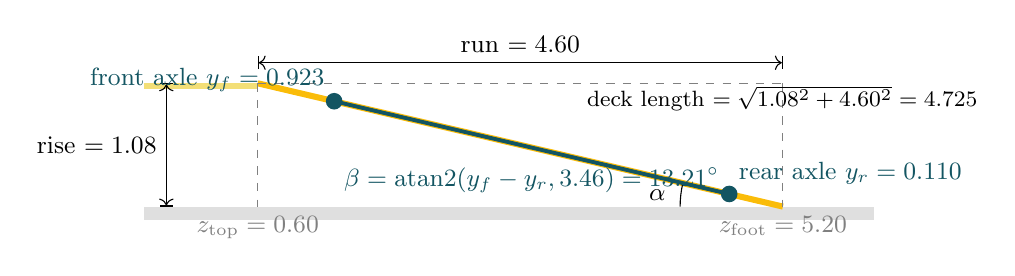
\begin{tikzpicture}[x=1.45cm, y=1.45cm, font=\small]
  \def\zt{0.6} \def\zf{5.2} \def\top{1.08}
  \fill[gray!25] (-0.4,-0.12) rectangle (6.0,0);
  \fill[yellow!45!smamber!60] (-0.4,\top-0.05) rectangle (\zt,\top);
  \draw[line width=2.2pt, yellow!50!orange] (\zt,\top) -- (\zf,0);
  \draw[dashed, gray] (\zt,\top) -- (\zt,0) node[below]{$z_{\text{top}}=0.60$};
  \draw[dashed, gray] (\zf,\top) -- (\zf,0) node[below]{$z_{\text{foot}}=5.20$};
  \draw[dashed, gray] (\zt,\top) -- (\zf,\top);
  \draw[|<->|] (\zt,\top+0.18) -- (\zf,\top+0.18) node[midway,above]{run $=4.60$};
  \draw[|<->|] (-0.2,0) -- (-0.2,\top) node[midway,left]{rise $=1.08$};
  \draw (\zf-0.9,0) arc (180:166.8:0.9) node[midway,left=2pt]{$\alpha$};
  \node[above right, font=\footnotesize] at (3.4,0.75) {deck length $=\sqrt{1.08^2+4.60^2}=4.725$};
  % vehicle axles at z = 3.0 -/+ 1.73 (front toward smaller z)
  \pgfmathsetmacro{\yf}{1.08*(5.2-1.27)/4.6}
  \pgfmathsetmacro{\yr}{1.08*(5.2-4.73)/4.6}
  \draw[smcyan!50!black, line width=1.4pt] (1.27,\yf) -- (4.73,\yr);
  \fill[smcyan!50!black] (1.27,\yf) circle (3pt) node[above left]{front axle $y_f=0.923$};
  \fill[smcyan!50!black] (4.73,\yr) circle (3pt) node[above right]{rear axle $y_r=0.110$};
  \node[smcyan!50!black, below=3pt] at (3.0,0.50) {$\beta=\operatorname{atan2}(y_f-y_r,3.46)=13.21^\circ$};
\end{tikzpicture}
}\end{minipage}\hfill
\begin{minipage}[c]{0.25\textwidth}\shot{\linewidth}{images/objects/ramp.jpg}\end{minipage}\hfill
\begin{minipage}[c]{0.25\textwidth}\shot{\linewidth}{images/objects/turntable.jpg}\end{minipage}
\caption{Ramp profile of Eq.~\eqref{eq:ramp} with the vehicle at $z=3.0$ (left); rendered ramp (middle) and turntable at $\psi=40^\circ$ (right).}\label{fig:ramp}
\end{figure}
\viva{Approach ramp (slope) and turntable}{\fn{SceneObjects.cpp}, \fn{Main.cpp}}{\fn{drawLiftApproachRamp()}, \fn{drawScene()}, \fn{moveCarYawToward()}}
{\fn{LIFT\_RAMP\_LEN}=4.60, rise $1.08$, slope $13.21^\circ$, deck $4.725$, \fn{LIFT\_TRACK}=0.98, \fn{TURN\_D}=4.20, \fn{carYaw}, $34^\circ$/s}
{a longer \fn{LIFT\_RAMP\_LEN} lowers the slope $\alpha$ (gentler but longer); a taller platform makes it steeper; a larger \fn{TURN\_D} widens the plate (it must stay within the lift base); a larger turn rate spins the car faster.}
{Eq.~\eqref{eq:ramp}; Fig.~\ref{fig:ramp}}

% ---------------------------------------------------------------- hoses
\subsection{B\'ezier hydraulic hoses}
Each hose is a tube swept along a cubic curve (the project's only equation-defined geometry):
\begin{equation}\begin{gathered}B(t)=(1-t)^3P_0+3(1-t)^2tP_1+3(1-t)t^2P_2+t^3P_3,\\
B'(t)=3(1-t)^2(P_1-P_0)+6(1-t)t(P_2-P_1)+3t^2(P_3-P_2).\end{gathered}\label{eq:bezier}\end{equation}
The curve is sampled at 14 points; each chord $B(t_{i-1})\to B(t_i)$ becomes a smooth cylinder aimed by $b=\arccos d_y$,
$a=\operatorname{atan2}(d_z,-d_x)$ ($d$ = unit chord direction), and a sphere at each knot hides the joints. For hose 0, $\text{bow}=0.55+0.30\,\text{hash01}(3)=0.727$ and the
control points of Fig.~\ref{fig:bezier} give $B(0.5)=0.125P_0+0.375P_1+0.375P_2+0.125P_3=(1.625,\,0.107,\,-0.705)$,
and the polyline length is \SI{3.12}{m}. For the chord $t\in[0.5,0.571]$ the direction is almost $+x$, so $b\approx91.7^\circ$, $a=180^\circ$: the cylinder is laid along the hose by $R_y(180^\circ)R_z(91.7^\circ)$.
\begin{figure}[!htbp]\centering
\begin{minipage}[c]{0.56\textwidth}\centering\resizebox{\linewidth}{!}{% Control polygon and curve of hydraulic hose 0 (top view, local x-z), values from drawLiftHydraulicHose().
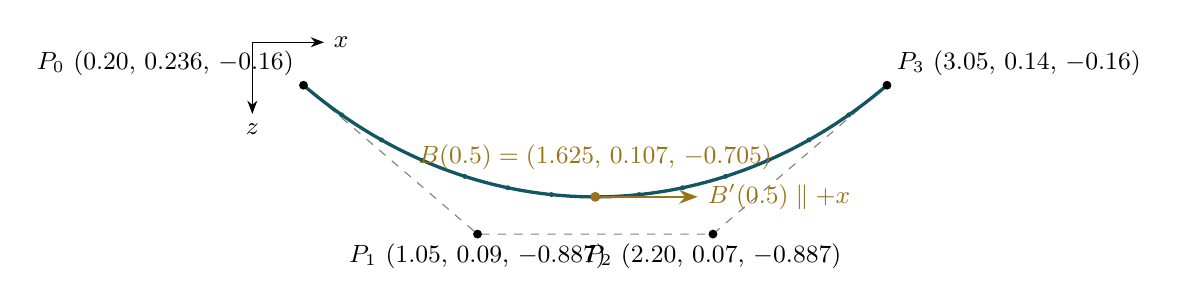
\begin{tikzpicture}[x=2.6cm, y=2.6cm, font=\small]
  \coordinate (P0) at (0.20,-0.160);
  \coordinate (P1) at (1.05,-0.887);
  \coordinate (P2) at (2.20,-0.887);
  \coordinate (P3) at (3.05,-0.160);
  \draw[gray, dashed] (P0) -- (P1) -- (P2) -- (P3);
  \draw[very thick, smcyan!50!black] (P0) .. controls (P1) and (P2) .. (P3);
  \foreach \t in {0.0714,0.1429,0.2143,0.2857,0.3571,0.4286,0.5,0.5714,0.6429,0.7143,0.7857,0.8571,0.9286}{
    \pgfmathsetmacro{\u}{1-\t}
    \pgfmathsetmacro{\bx}{\u^3*0.20+3*\u^2*\t*1.05+3*\u*\t^2*2.20+\t^3*3.05}
    \pgfmathsetmacro{\bz}{\u^3*(-0.16)+3*\u^2*\t*(-0.887)+3*\u*\t^2*(-0.887)+\t^3*(-0.16)}
    \fill[smcyan!50!black] (\bx,\bz) circle (0.9pt);}
  \fill (P0) circle (1.6pt) node[above left]{$P_0$ (0.20, 0.236, $-$0.16)};
  \fill (P1) circle (1.6pt) node[below]{$P_1$ (1.05, 0.09, $-$0.887)};
  \fill (P2) circle (1.6pt) node[below]{$P_2$ (2.20, 0.07, $-$0.887)};
  \fill (P3) circle (1.6pt) node[above right]{$P_3$ (3.05, 0.14, $-$0.16)};
  \fill[smamber!70!black] (1.625,-0.705) circle (1.8pt);
  \draw[-{Stealth}, smamber!70!black, thick] (1.625,-0.705) -- ++(0.5,0) node[right]{$B'(0.5)\parallel{+}x$};
  \node[above, smamber!70!black] at (1.625,-0.62) {$B(0.5)=(1.625,\,0.107,\,-0.705)$};
  \draw[-{Stealth}] (-0.05,0.05) -- (0.3,0.05) node[right]{$x$};
  \draw[-{Stealth}] (-0.05,0.05) -- (-0.05,-0.30) node[below]{$z$};
\end{tikzpicture}
}\end{minipage}\hfill
\begin{minipage}[c]{0.42\textwidth}\centering\shot{\linewidth}{images/lift/bezier_hoses.jpg}\\[2pt]\shot{\linewidth}{images/lift/bezier_hoses_wire.jpg}\end{minipage}
\caption{Control polygon and samples of hose 0 with $B(0.5)$ and its tangent (left); rendered hoses, shaded and wireframe (right).}\label{fig:bezier}
\end{figure}
\viva{B\'ezier hose}{\fn{SceneObjects.cpp}}{\fn{drawLiftHydraulicHose()}, \fn{drawBezierHose()}, \fn{drawTubeSegment()}}
{14 segments, radius 0.045, $P_0=(0.20,0.236,\mp0.16)$, $P_3=(3.05,0.14,\mp0.16)$, \fn{bow}=0.727}
{raising the control points' $y$ lifts the sag; a larger \fn{bow} pushes the loop outward; more segments give a smoother tube at more draw calls.}
{Eq.~\eqref{eq:bezier}; Fig.~\ref{fig:bezier}}

% ---------------------------------------------------------------- shell and props
\subsection{Garage shell and furniture: workbench, work stool, racking, oil drums}\label{sec:props}
\textbf{The shell.} Every shell part is one scaled cube and all sizes are constants (\fn{GARAGE\_W}=28, \fn{GARAGE\_D}=26, \fn{GARAGE\_H}=7, \fn{WALL\_T}=0.4):
\begin{align}
M_{\text{floor}}&=T(0,-0.15,0)\,S(28.8,0.30,26.8), & M_{\text{back wall}}&=T(0,3.5,-13.2)\,S(28.8,7.0,0.4),\nonumber\\
M_{\text{post}}&=T(\pm10.45,3.5,13.2)\,S(7.9,7.0,0.5), & 7.9&=\tfrac12(28.8-13),\;\;10.45=\tfrac{13}{2}+\tfrac{7.9}{2}.\label{eq:shell}
\end{align}
The floor top is at $y=0$ because the centre is $-0.15$ for thickness $0.30$; the posts leave exactly the $13$ m door opening. Outside, a $20\times6$ m apron where the car waits is followed by an $8$ m road with centre and edge lines, boundary walls with piers on both sides and at the back, and open ground to the horizon. There are no street lamps; key \fn{0} switches the exterior between constant daylight and night.
\textbf{Furniture and props} use the same recipe: choose a primitive, scale it to the real size, translate it to its place (Fig.~\ref{fig:props}).
\begin{figure}[!htbp]\centering
\resizebox{0.98\textwidth}{!}{% prop dimensions drawn to scale (metres) from drawWorkbench / drawWorkStool; x=y=1.45cm per metre
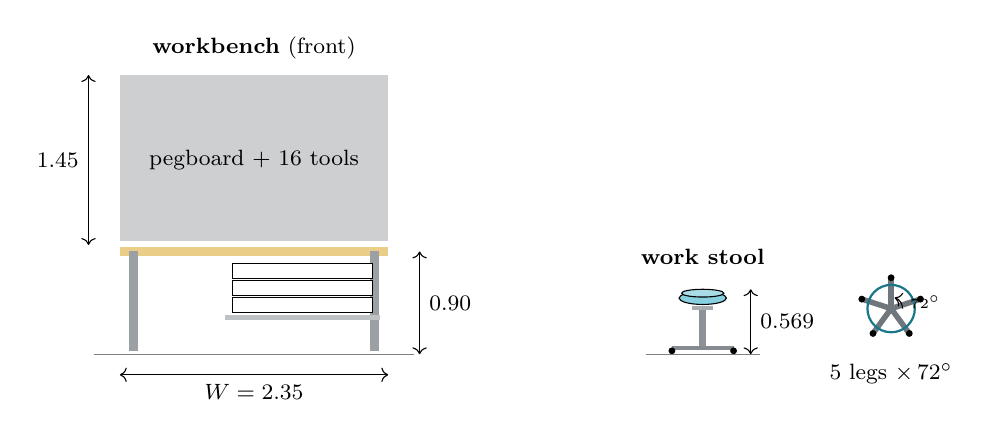
\begin{tikzpicture}[x=1.45cm,y=1.45cm,font=\footnotesize]
\begin{scope}[shift={(-1.18,0)}]
\draw[gray] (-1.4,0) -- (1.4,0);
\fill[smsteel!35] (-1.175,0.995) rectangle (1.175,2.445);
\fill[smamber!55] (-1.175,0.8575) rectangle (1.175,0.9425);
\fill[smsteel!70] (-1.0975,0.03) rectangle (-1.0175,0.9);
\fill[smsteel!70] (1.0175,0.03) rectangle (1.0975,0.9);
\fill[smsteel!45] (-0.2570,0.2975) rectangle (1.1030,0.3425);
\draw[fill=white] (-0.1880,0.3650) rectangle (1.0340,0.4950);
\draw[fill=white] (-0.1880,0.5150) rectangle (1.0340,0.6450);
\draw[fill=white] (-0.1880,0.6650) rectangle (1.0340,0.7950);
\draw[<->] (-1.175,-0.18) -- (1.175,-0.18) node[midway,below] {$W=2.35$};
\draw[<->] (1.45,0) -- (1.45,0.9) node[midway,right] {0.90};
\draw[<->] (-1.45,0.9575) -- (-1.45,2.445) node[midway,left] {1.45};
\node at (0,1.7) {pegboard + 16 tools};
\node[above] at (0,2.5) {\textbf{workbench} (front)};
\end{scope}
\begin{scope}[shift={(2.75,0)}]
\draw[gray] (-0.5,0) -- (0.5,0);
\fill[smsteel!80] (-0.03,0.035) rectangle (0.03,0.405);
\fill[smsteel!60] (-0.0925,0.385) rectangle (0.0925,0.425);
\fill[smsteel!85] (-0.27,0.035) rectangle (0.27,0.075);
\fill[black] (-0.270,0.03) circle (0.03);
\fill[black] (0.270,0.03) circle (0.03);
\draw[fill=smcyan!55] (0,0.492) ellipse (0.2075 and 0.056);
\draw[fill=smcyan!40] (0,0.535) ellipse (0.185 and 0.034);
\draw[<->] (0.42,0) -- (0.42,0.569) node[midway,right] {0.569};
\node[above] at (0,0.7) {\textbf{work stool}};
\end{scope}
\begin{scope}[shift={(4.4,0.4)}]
\draw[line width=2pt,smsteel] (0,0) -- (0.000,0.270);
\fill[black] (0.000,0.270) circle (0.03);
\draw[line width=2pt,smsteel] (0,0) -- (-0.257,0.083);
\fill[black] (-0.257,0.083) circle (0.03);
\draw[line width=2pt,smsteel] (0,0) -- (-0.159,-0.218);
\fill[black] (-0.159,-0.218) circle (0.03);
\draw[line width=2pt,smsteel] (0,0) -- (0.159,-0.218);
\fill[black] (0.159,-0.218) circle (0.03);
\draw[line width=2pt,smsteel] (0,0) -- (0.257,0.083);
\fill[black] (0.257,0.083) circle (0.03);
\draw[smcyan!70!black,thick] (0,0) circle (0.2075);
\draw[->] (0.1,0) arc (0:72:0.1) node[midway,right] {\tiny72$^\circ$};
\node[below] at (0,-0.4) {5 legs $\times\,72^\circ$};
\end{scope}
\end{tikzpicture}
}\\[3pt]
\begin{subfigure}{0.245\textwidth}\shot{\linewidth}{images/objects/workbench.jpg}\caption{Workbench}\end{subfigure}\hfill
\begin{subfigure}{0.245\textwidth}\shot{\linewidth}{images/objects/stool.jpg}\caption{Work stool (fabric)}\end{subfigure}\hfill
\begin{subfigure}{0.245\textwidth}\shot{\linewidth}{images/objects/drums.jpg}\caption{Oil drums}\end{subfigure}\hfill
\begin{subfigure}{0.245\textwidth}\shot{\linewidth}{images/objects/racking.jpg}\caption{Racking bay}\end{subfigure}
\caption{Dimensions (metres, to scale) of the workbench front and the work stool side and top view, taken from \fn{drawWorkbench} and \fn{drawWorkStool}; below, the rendered props (the oil drums beside the inside entrance wall).}\label{fig:props}
\end{figure}
\textbf{Workbench} (\fn{drawWorkbench}, three in the garage). A timber top $S(2.35,0.085,0.78)$ at $y=0.90$ on four legs $S(0.08,0.87,0.08)$ placed at $x=\pm W\cdot0.45=\pm1.0575$, $z=\pm D\cdot0.35=\pm0.273$;
a lower shelf $S(1.36,0.045,0.67)$ at $y=0.32$ and three drawers $S(1.22,0.13,0.03)$ at $y=0.43,\,0.58,\,0.73$ under the right-hand end. Behind it a pegboard $S(2.35,1.45,0.04)$ is centred at
$y=0.90+0.82=1.72$ (spans $0.995$--$2.445$) with a $14\times6$ grid of peg holes at $x=(c-6.5)\cdot0.155$, $y=1.25+0.225\,r$, and 16 hanging tools at $x=(i-7.5)\cdot0.142$ whose heights are varied by a deterministic hash.\\
\textbf{Work stool} (\fn{drawWorkStool}, four in the garage; the ``chair''). Seat height: two flattened UV spheres, the lower cushion $S(0.415,0.112,0.415)$ at $y=0.492$ (semi-axes $0.2075,\,0.056$) and the upper cushion
$S(0.370,0.068,0.370)$ at $y=0.535$, so the top of the seat is $0.535+0.034=0.569$ m. Under the seat: a seat plate $\varnothing\,0.185$ at $y=0.405$, a chrome gas post $\varnothing\,0.07$ from $0.035$ to $0.405$, and
\textbf{five legs} $S(0.27,0.04,0.048)$ at $(0.145,0.055,0)$, each rotated $R_y(72^\circ i)$ with $72^\circ=360^\circ/5$, ending in a rubber castor at radius $0.27$ (footprint $\approx\varnothing\,0.60$). The cushion uses the
\emph{woven-fabric} material (\fn{MAT\_FABRIC}): fully diffuse (roughness $0.97$), a thread weave of $\sin(420(x+0.7y))\cdot\sin(420(z-0.7y))$ (a $1.5$ cm repeat measured in world metres, faded out when a pixel is wider than half a thread), a fibre fuzz and a piped
seam with a tufting button --- so it reads as soft upholstery, not plastic.\\
\textbf{Oil drums} (\fn{drawOilDrum}, twelve). Each drum is one smooth cylinder with pressed ribs and rims. All twelve are stored as a staggered $3\times4$ block \emph{beside the inside entrance wall} ($x=10.0$--$12.6$, $z=8.5$--$12.4$), outside the $13$ m door opening, so the drive path, the lift and the rear work zone stay clear.\\
\textbf{Racking bay} (\fn{drawRackingBay}). Width $2.70$, depth $1.05$, level spacing $1.32$: height $H=1.32n+0.30$ ($4.26$ for $n=3$), uprights at $x=\pm1.35$, $z=\pm0.399$, beams at $y=0.45+1.32L=0.45,\,1.77,\,3.09$, diagonal bracing at $\pm38^\circ$.
\viva{Workbench}{\fn{SceneObjects.cpp}}{\fn{drawWorkbench(parent, index)}; placed in \fn{drawScene()} at $(-3.0,0,-12.1)$, $(2.7,0,-12.1)$, $(12.72,0,-1.6)$}
{$W=2.35$, $D=0.78$, \fn{TOP\_Y}=0.90, legs $\pm1.0575,\pm0.273$, pegboard centre $y=1.72$ (1.45 high), 16 tools}
{raising \fn{TOP\_Y} lifts the top (legs and pegboard follow because they are written relative to it); a larger $W$ widens the top, leg spacing and pegboard together; changing the hash seed re-arranges the hanging tools.}
{Fig.~\ref{fig:props}}
\viva{Work stool (chair)}{\fn{SceneObjects.cpp}, \fn{Shader.cpp}}{\fn{drawWorkStool(parent, index)}; fabric branch \fn{uMaterialType == 21} in \fn{materialMaps()}}
{seat $S(0.415,0.112,0.415)$ at $0.492$ and $S(0.370,0.068,0.370)$ at $0.535$ (top $0.569$), gas post $\varnothing\,0.07$, 5 legs $\times72^\circ$ of length $0.27$, roughness $0.97$, weave repeat 1.5 cm}
{moving the cushion $y$ changes the seat height (the post length must follow); more or fewer than 5 legs needs $360^\circ/n$; lowering the roughness would make the cushion shiny again; the weave frequency (420) sets the thread size.}
{Fig.~\ref{fig:props}}


% =====================================================================
\section{Transformations, Camera and Projection}\label{sec:transform}
\textbf{Model matrix.} Points are homogeneous, $\vect p'=M\vect p$. \fn{Scene::place(pos,size,rot)} builds
\begin{equation}M=T\,R_y R_x R_z\,S,\quad
T=\begin{bmatrix}1&0&0&t_x\\0&1&0&t_y\\0&0&1&t_z\\0&0&0&1\end{bmatrix},\;
S=\operatorname{diag}(s_x,s_y,s_z,1),\;
R_x=\begin{bmatrix}1&0&0&0\\0&c&-s&0\\0&s&c&0\\0&0&0&1\end{bmatrix}\label{eq:trs}\end{equation}
($R_y$, $R_z$ analogous; \fn{Math3D.h} stores column-major). Read right-to-left: scale the unit cube, rotate it about
its own centre, then translate (Fig.~\ref{fig:trs}). \emph{Example} (floor): $M=T(0,-0.15,0)S(28.8,0.3,26.8)$ maps the
corner $(0.5,0.5,0.5)$ to $(14.4,0,13.4)$: the slab top lies on $y=0$.
\begin{figure}[!htbp]\centering
\resizebox{0.92\textwidth}{!}{% Unit cube -> S -> R -> T for one scissor arm (drawScissorStack, h = 1.10 m, theta = 14.75 deg).
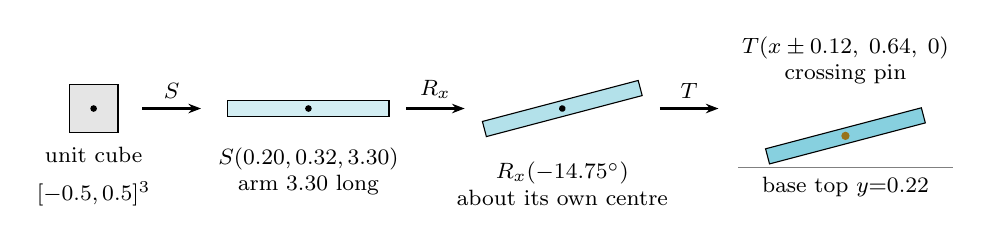
\begin{tikzpicture}[font=\footnotesize, x=0.62cm, y=0.62cm, arr/.style={-{Stealth[length=1.6mm]}, thick}]
  % 1 unit cube
  \begin{scope}[shift={(0,0)}]
    \draw[fill=gray!20] (-0.5,-0.5) rectangle (0.5,0.5);
    \fill (0,0) circle (1.2pt);
    \node[below] at (0,-0.6) {unit cube};
    \node[below, align=center] at (0,-1.3) {$[-0.5,0.5]^3$};
  \end{scope}
  \draw[arr] (1.0,0) -- (2.2,0) node[midway, above]{$S$};
  % 2 scaled (z horizontal = 3.30, y vertical = 0.32)
  \begin{scope}[shift={(4.4,0)}]
    \draw[fill=smcyan!20] (-1.65,-0.16) rectangle (1.65,0.16);
    \fill (0,0) circle (1.2pt);
    \node[below, align=center] at (0,-0.6) {$S(0.20,0.32,3.30)$\\ arm $3.30$ long};
  \end{scope}
  \draw[arr] (6.4,0) -- (7.6,0) node[midway, above]{$R_x$};
  % 3 rotated by -theta about its centre
  \begin{scope}[shift={(9.6,0)}, rotate=14.75]
    \draw[fill=smcyan!35] (-1.65,-0.16) rectangle (1.65,0.16);
    \fill (0,0) circle (1.2pt);
  \end{scope}
  \node[below, align=center] at (9.6,-0.9) {$R_x(-14.75^\circ)$\\ about its own centre};
  \draw[arr] (11.6,0) -- (12.8,0) node[midway, above]{$T$};
  % 4 translated to the crossing point
  \draw[gray] (13.2,-1.2) -- (17.6,-1.2);
  \node[below] at (15.4,-1.2) {base top $y{=}0.22$};
  \begin{scope}[shift={(15.4,-1.2+0.64/0.62*0.62)}, rotate=14.75]
    \draw[fill=smcyan!55] (-1.65,-0.16) rectangle (1.65,0.16);
  \end{scope}
  \fill[smamber!70!black] (15.4,-1.2+0.64) circle (1.5pt);
  \node[above, align=center] at (15.4,0.3) {$T(x\pm0.12,\;0.64,\;0)$\\ crossing pin};
\end{tikzpicture}
}
\caption{Unit cube $\to$ scale $\to$ rotate $\to$ translate for one scissor arm at $h=1.10$\,m.}\label{fig:trs}
\end{figure}

\textbf{Hierarchy.} $M_{\text{child,world}}=M_{\text{parent,world}}M_{\text{child,local}}$ (Fig.~\ref{fig:hier}). The vehicle matrix
(\fn{serviceCarMatrix()}) is
\begin{equation}M_{\text{car}}=T(0,\;\text{\fn{liftTopY}}(h)+\Delta y,\;-2+18.5\,c)\;R_x(\beta)\;R_y(\psi),\label{eq:car}\end{equation}
$c$ = \fn{carDrive} (1 outside, 0 on lift), $\beta$ ramp pitch, $\psi$ turntable yaw. Changing $c$ moves the whole car and
every child with one number.
\begin{figure}[!htbp]\centering
\resizebox{0.95\textwidth}{!}{% Parent-child transformation trees (drawScene / drawCar / drawRobotArm); edge labels = controlling variable.
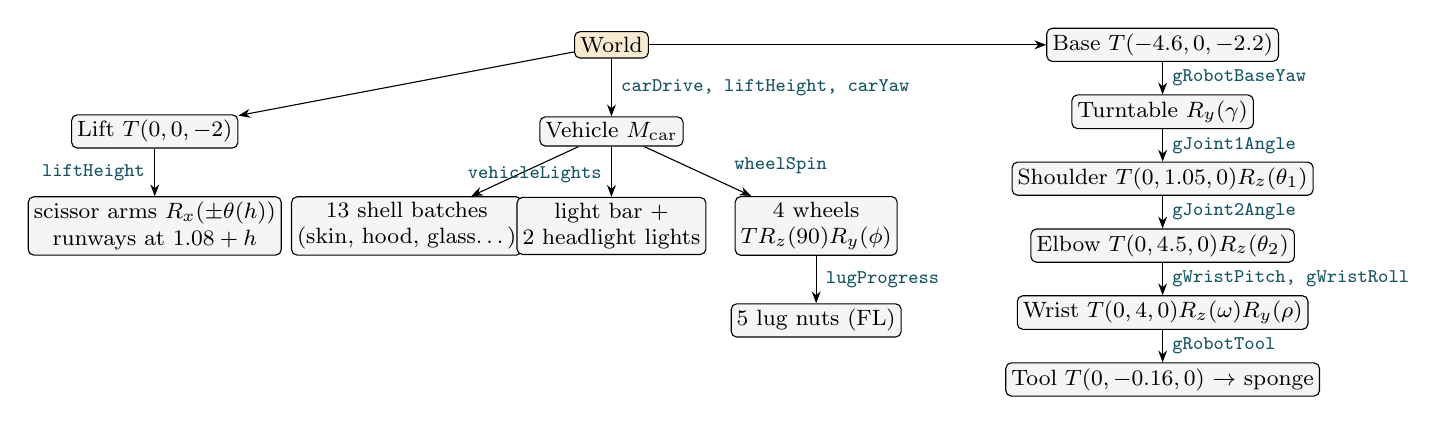
\begin{tikzpicture}[font=\footnotesize,
  n/.style={draw, rounded corners=2pt, fill=gray!8, inner sep=2pt, align=center},
  v/.style={font=\scriptsize\ttfamily, text=smcyan!50!black},
  arr/.style={-{Stealth[length=1.5mm]}}]
  % ---------------- vehicle
  \node[n, fill=smamber!22] (W) at (0,0) {World};
  \node[n] (C) at (0,-1.1) {Vehicle $M_{\text{car}}$};
  \draw[arr] (W) -- node[v, right]{carDrive, liftHeight, carYaw} (C);
  \node[n] (S) at (-2.6,-2.3) {13 shell batches\\(skin, hood, glass\dots)};
  \node[n] (L) at (0,-2.3) {light bar +\\2 headlight lights};
  \node[n] (Wh) at (2.6,-2.3) {4 wheels\\$T R_z(90) R_y(\phi)$};
  \node[n] (Lg) at (2.6,-3.5) {5 lug nuts (FL)};
  \draw[arr] (C) -- (S); \draw[arr] (C) -- node[v, left, pos=0.55]{vehicleLights} (L);
  \draw[arr] (C) -- node[v, above right, pos=0.75]{wheelSpin} (Wh); \draw[arr] (Wh) -- node[v, right]{lugProgress} (Lg);
  % ---------------- robot
  \node[n] (B) at (7.0,0) {Base $T(-4.6,0,-2.2)$};
  \node[n] (Tt) at (7.0,-0.85) {Turntable $R_y(\gamma)$};
  \node[n] (Sh) at (7.0,-1.7) {Shoulder $T(0,1.05,0)R_z(\theta_1)$};
  \node[n] (El) at (7.0,-2.55) {Elbow $T(0,4.5,0)R_z(\theta_2)$};
  \node[n] (Wr) at (7.0,-3.4) {Wrist $T(0,4,0)R_z(\omega)R_y(\rho)$};
  \node[n] (To) at (7.0,-4.25) {Tool $T(0,-0.16,0)$ $\to$ sponge};
  \draw[arr] (W) -- (B);
  \draw[arr] (B) -- node[v, right]{gRobotBaseYaw} (Tt);
  \draw[arr] (Tt) -- node[v, right]{gJoint1Angle} (Sh);
  \draw[arr] (Sh) -- node[v, right]{gJoint2Angle} (El);
  \draw[arr] (El) -- node[v, right]{gWristPitch, gWristRoll} (Wr);
  \draw[arr] (Wr) -- node[v, right]{gRobotTool} (To);
  % ---------------- lift
  \node[n] (Li) at (-5.8,-1.1) {Lift $T(0,0,-2)$};
  \node[n] (Sc) at (-5.8,-2.3) {scissor arms $R_x(\pm\theta(h))$\\runways at $1.08+h$};
  \draw[arr] (W) -- (Li); \draw[arr] (Li) -- node[v, left]{liftHeight} (Sc);
\end{tikzpicture}
}
\caption{Parent--child transformation trees; blue labels are the variables that drive each edge.}\label{fig:hier}
\end{figure}

\textbf{Normal matrix.} Under non-uniform scale, normals use $N=(M_{3\times3}^{-1})^T$ (\fn{normalMatrix()}); for the floor
$N=\operatorname{diag}(1/28.8,1/0.3,1/26.8)$, and the top normal stays $(0,1,0)$ after normalisation.

\textbf{Camera / view.} $\vect f=(\cos\psi\cos\varphi,\sin\varphi,\sin\psi\cos\varphi)$, $\vect r=\widehat{\vect f\times\vect y}$;
\fn{lookAt(eye, eye+f, up)} moves the world so the eye is at the origin looking down $-z$. Speed \SI{7}{m/s}
(\fn{moveSpeed}), mouse \SI{0.1}{\degree/px}, FOV 20--90$^\circ$ by scroll.

\textbf{Projection.} Perspective ($f=1/\tan(\text{fov}/2)$, $a$ = aspect, $z_n=0.05$, $z_f=200$) and orthographic:
\begin{equation}P=\begin{bmatrix}f/a&0&0&0\\0&f&0&0\\0&0&\frac{z_f+z_n}{z_n-z_f}&\frac{2z_fz_n}{z_n-z_f}\\0&0&-1&0\end{bmatrix},\qquad
O=\begin{bmatrix}\frac{2}{r-l}&0&0&-\frac{r+l}{r-l}\\0&\frac{2}{t-b}&0&-\frac{t+b}{t-b}\\0&0&\frac{-2}{z_f-z_n}&-\frac{z_f+z_n}{z_f-z_n}\\0&0&0&1\end{bmatrix}.\label{eq:proj}\end{equation}
With fov $60^\circ$, $f=1.732$: a point at $x=1$ maps to $x_{ndc}=0.195$ at depth 5 and $0.049$ at depth 20 (smaller when
farther). \fn{Backspace} switches to $O$ with $t=d\tan(\text{fov}/2)$ at the vehicle distance $d$, so only the
projection changes (Fig.~\ref{fig:proj}).
\begin{figure}[!htbp]\centering
\begin{subfigure}{0.48\textwidth}\shot{\linewidth}{images/comparisons/perspective.jpg}\caption{Perspective: runway edges converge}\end{subfigure}\hfill
\begin{subfigure}{0.48\textwidth}\shot{\linewidth}{images/comparisons/orthographic.jpg}\caption{Orthographic: edges stay parallel}\end{subfigure}
\caption{Projection switch (\fn{Backspace}): same camera position, direction and field of view; only the projection matrix changes.}\label{fig:proj}
\end{figure}
\viva{Camera and projection}{\fn{Math3D.h}, \fn{Camera.h}, \fn{Main.cpp}}{\fn{perspective()}, \fn{orthographic()}, \fn{lookAt()}, \fn{Camera::viewMatrix()}, render loop in \fn{main()}}
{\fn{gCamera.fov}=60$^\circ$ (20--90), near 0.05, far 200, \fn{moveSpeed}=7.0, \fn{mouseSens}=0.10, start $(4.6,2.9,10.2)$, yaw $-104^\circ$, pitch $-8^\circ$, \fn{gOrthographic}}
{smaller fov zooms in (larger $f$); a larger near plane clips close objects; far plane $<$ scene size clips the far wall; \fn{gOrthographic}=true removes the perspective division.}
{Eq.~\eqref{eq:proj}; Fig.~\ref{fig:proj}}

% =====================================================================
\section{Lighting, Shading, Materials and Textures}\label{sec:lighting}
\subsection{Phong lighting model (course theory, as implemented)}
\begin{center}\fcolorbox{smamber}{smamber!6}{\begin{minipage}{0.92\linewidth}\centering
$\displaystyle I=I_a+I_d+I_s,\qquad I_a=k_aL_a,\qquad I_d=k_dL_d\max(\vect N\!\cdot\!\vect L,0),\qquad I_s=k_sL_s\max(\vect R\!\cdot\!\vect V,0)^{n}$\\[2pt]
{\scriptsize ambient: base light on every surface \;|\; diffuse: depends on the angle between normal and light \;|\; specular: highlight, sharper for larger $n$}
\end{minipage}}\end{center}
\fn{phongReflection()} in \fn{Shader.cpp} implements the classical Phong reflection model~\cite{phong1975} for every
light $j$ (directional, up to 10 point lights, spotlight):
\begin{equation}
I=\underbrace{k_aL_a}_{\text{ambient}}+\sum_j A_j\Big[\underbrace{k_d L_j\max(\vect N\cdot\vect L_j,0)}_{\text{diffuse}}
+\underbrace{k_s L_j\max(\vect R_j\cdot\vect V,0)^{n}}_{\text{specular}}\Big],\qquad \vect R_j=\operatorname{reflect}(-\vect L_j,\vect N).
\label{eq:phong}\end{equation}
Project values: $k_aL_a=0.038$; $k_d$ = material albedo (diffuse reduced by $0.30$--$0.35\,m$ for metals); $k_s=\operatorname{mix}(0.12,0.75,m)$
(directional), $\operatorname{mix}(0.08,0.48,m)$ (point), $\operatorname{mix}(0.10,0.55,m)$ (spot); shininess $n=\operatorname{mix}(180,10,r)$ from
roughness $r$; point attenuation $A=1/(1+0.075d+0.018d^2)$; final colour $C=k_d\odot I_{a+d}+I_s\cdot\operatorname{mix}(1,k_d,m)$.
\begin{lstlisting}
float n = mix(180.0, 10.0, clamp(rough, 0.04, 1.0));          // shininess
diffuse = vec3(0.038);                                         // ambient  ka*La
vec3 L = normalize(-uDirLightDirection);  vec3 R = reflect(-L, N);
diffuse  += Ldir * max(dot(N, L), 0.0) * (1.0 - 0.35 * metal);                  // kd*Ld*max(N.L,0)
specular += Ldir * pow(max(dot(R, V), 0.0), n) * mix(0.12, 0.75, metal);         // ks*Ls*max(R.V,0)^n
\end{lstlisting}
\emph{Example}: a plastic surface ($m=0$, $r=0.58$) has $n=\operatorname{mix}(180,10,0.58)=81.4$ and $k_s=0.12$ for the sun; a point light
\SI{6.59}{m} away is attenuated to $A=1/(1+0.494+0.782)=0.44$.

\subsection{Gouraud versus Phong shading}
\textbf{Gouraud} (\fn{F5} once): Eq.~\eqref{eq:phong} is evaluated in the \emph{vertex} shader, which outputs \fn{vGouraudDiffuse}
and \fn{vGouraudSpecular}; the rasteriser interpolates them: $C_f=\alpha C_1+\beta C_2+\gamma C_3$ (barycentric,
$\alpha+\beta+\gamma=1$)~\cite{gouraud1971}. \textbf{Phong} (\fn{F5} twice): the \emph{normal} is interpolated and the same
function runs per \emph{fragment}, with shadows. The floor slab is only two triangles, so under Gouraud a spotlight or
headlight pool that falls between its vertices disappears, while Phong reproduces it (Fig.~\ref{fig:shading}).
\begin{figure}[!htbp]\centering
\begin{subfigure}{0.49\textwidth}\shot{\linewidth}{images/shading/spot_gouraud.jpg}\caption{Gouraud: spotlight pool lost}\end{subfigure}\hfill
\begin{subfigure}{0.49\textwidth}\shot{\linewidth}{images/shading/spot_phong.jpg}\caption{Phong: crisp spotlight pool}\end{subfigure}\\[2pt]
\begin{subfigure}{0.49\textwidth}\shot{\linewidth}{images/shading/headlight_gouraud.jpg}\caption{Gouraud: no headlight falloff}\end{subfigure}\hfill
\begin{subfigure}{0.49\textwidth}\shot{\linewidth}{images/shading/headlight_phong.jpg}\caption{Phong: headlight point-light pool}\end{subfigure}\\[2pt]
\begin{subfigure}{0.49\textwidth}\shot{\linewidth}{images/shading/spot_pbr.jpg}\caption{PBR: soft spotlight (reference)}\end{subfigure}\hfill
\begin{subfigure}{0.49\textwidth}\shot{\linewidth}{images/lighting/headlights_off.jpg}\caption{Headlights off (key \fn{'})}\end{subfigure}
\caption{\textbf{Gouraud Shading Mode} vs \textbf{Phong Shading Mode} vs PBR, ceiling lights off to isolate the scanner spotlight (a, b, e) and the headlight point lights (c, d, f).}\label{fig:shading}
\end{figure}
\viva{Phong / Gouraud shading}{\fn{Shader.cpp}, \fn{Main.cpp}}{\fn{phongReflection()}, fragment \fn{main()}, key \fn{F5} in \fn{handleDiscreteKey()}}
{\fn{uShadingMode} = 0 PBR / 1 Gouraud / 2 Phong; ambient 0.038; $n=\operatorname{mix}(180,10,r)$; $k_s$ as above}
{raising the ambient 0.038 brightens unlit sides; larger $n$ gives smaller, sharper highlights; larger $k_s$ brighter highlights; switching 1$\leftrightarrow$2 shows per-vertex vs per-fragment.}
{Eq.~\eqref{eq:phong}; Fig.~\ref{fig:shading}}

\subsection{Light types}
\begin{table}[!htbp]\centering\scriptsize
\caption{Light sources (all evaluated in \fn{phongReflection()} and \fn{pbrLighting()}).}\label{tab:lights}
\begin{tabular}{@{}l>{\raggedright}p{5.4cm}>{\raggedright}p{4.4cm}>{\raggedright\arraybackslash}p{2.6cm}@{}}\toprule
Light & Position / direction & Source & Control\\\midrule
Directional & $\hat{\vect d}=\widehat{(0.18,-1,-0.38)}$, colour $(0.95,0.91,0.84)$, $I=0.68$; $5{\times}5$ PCF shadow & \fn{buildLightSpaceMatrix()}, \fn{buildWorkshopRig()} & \fn{M} rigs, \fn{F8} shadows\\
Point (ceiling, 8) & $(\pm6.4,6.32,z_i)$, $z_i\in\{-10.1,-3.9,2.3,8.5\}$ (+0.55 right row), $I=1.28$ & \fn{buildWorkshopRig()} & \fn{;} (1.28 $\to$ 0.06)\\
Point (headlights, 2) & $M_{\text{car}}(\pm0.62,0.923,-2.735)$, $I=1.6$ & \fn{headlightLocalPosition()}, \fn{kHeadlightIntensity} & \fn{'}\\
Spotlight (moving) & at tool tip $\vect t$, direction $\widehat{\vect t-\vect w}$, cone $14^\circ/23^\circ$, $I=4.6$ cyan & \fn{uploadSceneUniforms()} & robot keys, \fn{F1}\\\bottomrule
\end{tabular}
\end{table}
Spotlight cone: $I_{\text{cone}}=\operatorname{clamp}\big(\frac{\cos\theta-\cos23^\circ}{\cos14^\circ-\cos23^\circ},0,1\big)$ with
$\cos\theta=-\vect L\cdot\hat{\vect s}$ (squared in PBR); at $18^\circ$ off-axis the weight is 0.614. Because $\vect t,\vect w$ come
from the joint angles each frame, it is a \emph{moving light}.
\viva{Lighting rig}{\fn{Main.cpp}, \fn{SceneObjects.cpp}}{\fn{buildWorkshopRig()}, \fn{buildLightSpaceMatrix()}, \fn{uploadSceneUniforms()}}
{\fn{bayLevel}=1.28, light $y=6.32$; sun $(0.18,-1,-0.38)$, \fn{keyIntensity}=0.68; spot cone $14^\circ/23^\circ$, $I=4.6$; \fn{kHeadlightIntensity}=1.6; key \fn{0}: night = moon $0.05$}
{moving a $z_i$ moves its light pool; raising \fn{bayLevel} brightens the room; widening the outer cone enlarges the spot; changing the sun vector rotates every shadow.}
{Eq.~\eqref{eq:phong}; Table~\ref{tab:lights}}

\subsection{Advanced extensions: PBR, shadows, textures, post-processing}
\textbf{Cook--Torrance PBR} (default; \fn{F5} cycles back to it): $f_r=\frac{k_d\,c}{\pi}+\frac{DFG}{4(\vect n\cdot\vect v)(\vect n\cdot\vect l)}$ with a
GGX distribution ($\alpha=r^2$), Schlick Fresnel and Smith geometry~\cite{cook1982reflectance,karis2013ue4}, anisotropic GGX on the stainless body, a clear-coat lobe and
split-sum image-based lighting. \textbf{Shadows:} a $2048^2$ directional map with $5{\times}5$ PCF (shadowed if $z-b>d_{\text{map}}$) and a $1024^2$ spot map that follows the
scanner~\cite{williams1978shadows}. \textbf{Textures:} a 4-layer \fn{GL\_TEXTURE\_2D\_ARRAY} (concrete, plaster, asphalt, tread plate) sampled by triplanar mapping,
weights $\vect w=|\vect n|^6/\|\cdot\|_1$, scale \fn{textureScaleFor()} (concrete 0.34). \textbf{Post-processing:} RGB16F HDR with 4$\times$MSAA, half-resolution bloom
(6 passes) and ACES tone mapping~\cite{narkowicz2016aces}.
\begin{figure}[!htbp]\centering
\begin{subfigure}{0.32\textwidth}\shot{\linewidth}{images/comparisons/shadows_on.jpg}\caption{Directional light + shadows}\end{subfigure}\hfill
\begin{subfigure}{0.32\textwidth}\shot{\linewidth}{images/lighting/ceiling_lights_off.jpg}\caption{Ceiling lights off (\fn{;})}\end{subfigure}\hfill
\begin{subfigure}{0.32\textwidth}\shot{\linewidth}{images/lighting/spotlight_night.jpg}\caption{Moving spotlight (night rig)}\end{subfigure}
\caption{Light types and shadows (the same views with shadows off, \fn{F8}, and textures off, \fn{F6}, are in the program).}\label{fig:lights}
\end{figure}
\subsection{Dirt, cleaning, polishing and the changing reflection}\label{sec:polish}
\textbf{The idea in one paragraph.} The vehicle carries two numbers that the service changes over time: \fn{dirtAmount} $D$ ($1\to0$, grime on the left flank) and \fn{polishAmount} $p$ ($0\to1$, finish of the whole steel shell).
The robot's \emph{sponge} lowers $D$ as it wipes; the robot's \emph{polisher} raises $p$ as it buffs. The fragment shader reads $D$ and $p$ every frame and changes how every pixel of the body is lit, so what you see
changes with the tool. No texture is repainted: it is a change in the \emph{material} (colour, roughness, metallic), and reflections follow automatically from the lighting equations.
\textbf{1. Cleaning (the sponge).} In state CLEAN the sponge follows three bands of 4 waypoints each (high, middle, low; \fn{PATH\_CLEAN\_HIGH/MID/LOW}). The dirt retreats \emph{in step with the sponge's position}:
$D=D_0-\Delta\cdot\text{pathProgress}$, where pathProgress $=\text{waypoint}/(4-1)$. The three bands take $D$ from $1\to0.65\to0.30\to0$ (code: \fn{gServiceVisual.dirtAmount}), so the clean band follows the tool instead of fading on a timer.
\textbf{2. How dirt is drawn (fragment shader).} A grime mask is built in the \emph{vehicle's own frame} (so it stays on the panel when the car is lifted): it sits on the serviced flank only, collects low and thins upward
(thrown up by the wheels), is heaviest behind the wheels, and is blotchy and streaked:
\begin{equation}\begin{gathered}\text{mask}=\text{clamp}\big(\;\underbrace{\text{side}\cdot\text{low}\cdot\text{along}}_{\text{where}}\cdot(0.35+0.95\,\text{blotch})(0.65+0.60\,\text{streak})\cdot D\cdot2.25,\;0,\,1\big),\\
\text{low}=1-\operatorname{smoothstep}(0.48,\,1.26,\,y_{\text{local}}).\end{gathered}\label{eq:dirt}\end{equation}
Where the mask is $m$: albedo $\leftarrow\operatorname{mix}(\text{albedo},\text{grime},0.88\,m)$ with grime $=(0.205,0.183,0.158)$; roughness $\leftarrow\operatorname{mix}(r,0.94,m)$; metallic $\leftarrow\text{metal}\,(1-0.92\,m)$; brushed grain and clear coat $\leftarrow(1-m)$.
The key point is the \textbf{metallic} term: dirt is a dielectric, so where the film is thick the surface stops behaving like a mirror --- that is why grime \emph{kills} a reflection instead of just tinting it.
\emph{Worked example} at height $y=0.8$ ($\text{low}=0.633$), blotch $=$ streak $=0.5$, $r=0.40$, metal $=0.97$:
\begin{center}\scriptsize\begin{tabular}{@{}rrrrr@{}}\toprule $D$ & mask $m$ & roughness & metallic & grime weight $0.88m$\\\midrule
1.00 (dirty) & 1.000 & 0.940 & 0.078 & 0.880\\ 0.65 (after high band) & 0.726 & 0.792 & 0.322 & 0.639\\ 0.30 (after middle band) & 0.335 & 0.581 & 0.671 & 0.295\\ 0.00 (clean) & 0 & 0.400 & 0.970 & 0\\\bottomrule\end{tabular}\end{center}
\textbf{3. Polishing (the polisher).} In state POLISH the buffer pad (\O\,0.58, spinning at $620^\circ$/s) makes six passes: high, middle and low band on the near flank, then the \emph{turntable turns the car $180^\circ$} and the same three bands
are polished on the far flank. $p$ rises $0.17,\,0.34,\,0.50,\,0.67,\,0.84,\,1.00$ pass by pass, so the shine spreads as the pad moves. All steel batches of the shell take the same finish (\fn{setSurfaceFinish(p)}), so a serviced car is polished all over.
\textbf{4. What polishing changes in the shader.} Three things, in this order:
\begin{equation}r'=\operatorname{mix}(r,\;0.34\,r+0.03,\;p)=r-p\,(r-0.166),\qquad \text{aniso}'=\text{aniso}\cdot(1-0.58\,p),\qquad \text{albedo}'=\text{albedo}\cdot(1+0.05\,p).\label{eq:polish}\end{equation}
With $r=0.40$ (as-rolled stainless) the roughness falls to $0.166$ at $p=1$, the brushed-grain directionality is cut to $42\%$, and the reflectance rises $5\%$ (the dull oxide layer is cut away). No lacquer is added: a coat belongs to the material, not to how hard it was buffed.
\textbf{5. Why the reflection changes.} Roughness enters the reflection in three places, and the table shows each for the three polish levels:
\begin{center}\scriptsize\begin{tabular}{@{}lccccc@{}}\toprule
$p$ & $r'$ & GGX peak $D_0$ & half-width & mip $6\sqrt{r'}$ & Phong $n$\\\midrule
0 (as rolled) & 0.400 & 12.4 & $5.99^\circ$ & 3.79 & 112\\ 0.5 & 0.283 & 49.6 & $2.96^\circ$ & 3.19 & 132\\ 1 (polished) & 0.166 & 419 & $1.02^\circ$ & 2.44 & 152\\\bottomrule\end{tabular}\end{center}
($D_0=1/(\pi r'^4)$ is the highlight peak, ``half-width'' the angle where $D$ falls to $D_0/2$, mip $=6\sqrt{r'}$ the cube-map level.) (a) \emph{Light highlights.} The GGX distribution $D(\theta_h)=\alpha^2/\big(\pi[\cos^2\!\theta_h(\alpha^2-1)+1]^2\big)$, $\alpha=r'^2$, becomes $34$ times higher and about six times narrower: a broad glow turns into a small hard glint of the ceiling lights (Fig.~\ref{fig:material}f).
(b) \emph{Environment reflection.} The room is a cube map with mip levels; the reflection ray reads level $6\sqrt{r'}$, so smaller $r'$ reads a \emph{sharper} mip and the reflected room becomes a clearer mirror image.
(c) \emph{Phong and Gouraud modes} use the shininess exponent $n=\operatorname{mix}(180,10,r')$, which rises from $112$ to $152$: the same sharpening appears when you press \fn{F5} --- the effect is a material change, not a PBR-only trick.
\begin{figure}[!htbp]\centering
\begin{subfigure}{0.32\textwidth}\shot{\linewidth}{images/polish/p1_dirty.jpg}\caption{Dirty, $D=1$, $p=0$}\end{subfigure}\hfill
\begin{subfigure}{0.32\textwidth}\shot{\linewidth}{images/polish/p2_half_clean.jpg}\caption{Half cleaned, $D=0.5$}\end{subfigure}\hfill
\begin{subfigure}{0.32\textwidth}\shot{\linewidth}{images/polish/p3_clean.jpg}\caption{Clean, $D=0$, $r=0.40$}\end{subfigure}\\[2pt]
\begin{subfigure}{0.32\textwidth}\shot{\linewidth}{images/polish/p4_half_polish.jpg}\caption{Half polished, $p=0.5$, $r'=0.283$}\end{subfigure}\hfill
\begin{subfigure}{0.32\textwidth}\shot{\linewidth}{images/polish/p5_polished.jpg}\caption{Polished, $p=1$, $r'=0.166$}\end{subfigure}\hfill
\begin{subfigure}{0.32\textwidth}\centering\resizebox{\linewidth}{!}{% GGX distribution D(theta_h)/D(0) for three roughness values (normalised highlight shape)
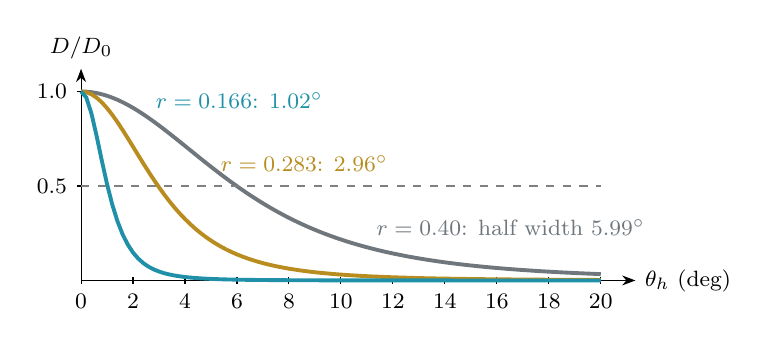
\begin{tikzpicture}[x=0.55cm,y=2.4cm,font=\footnotesize]
\draw[-{Stealth}] (0,0) -- (12.8,0) node[right] {$\theta_h$ (deg)};
\draw[-{Stealth}] (0,0) -- (0,1.12) node[above] {$D/D_0$};
\foreach \a in {0,2,4,...,20} {\draw (\a*0.6,0.02) -- (\a*0.6,-0.02) node[below] {\a};}
\foreach \y in {0.5,1.0} {\draw (0.1,\y) -- (-0.1,\y) node[left] {\y};}
\draw[color=smsteel,line width=1.4pt] plot coordinates {(0.000,1.0000) (0.120,0.9991) (0.240,0.9963) (0.360,0.9917) (0.480,0.9853) (0.600,0.9772) (0.720,0.9674) (0.840,0.9561) (0.960,0.9432) (1.080,0.9289) (1.200,0.9134) (1.320,0.8966) (1.440,0.8788) (1.560,0.8600) (1.680,0.8404) (1.800,0.8201) (1.920,0.7992) (2.040,0.7778) (2.160,0.7561) (2.280,0.7340) (2.400,0.7119) (2.520,0.6897) (2.640,0.6674) (2.760,0.6453) (2.880,0.6234) (3.000,0.6017) (3.120,0.5804) (3.240,0.5593) (3.360,0.5387) (3.480,0.5185) (3.600,0.4988) (3.720,0.4796) (3.840,0.4609) (3.960,0.4428) (4.080,0.4252) (4.200,0.4081) (4.320,0.3917) (4.440,0.3757) (4.560,0.3604) (4.680,0.3456) (4.800,0.3313) (4.920,0.3176) (5.040,0.3045) (5.160,0.2918) (5.280,0.2797) (5.400,0.2681) (5.520,0.2569) (5.640,0.2462) (5.760,0.2360) (5.880,0.2262) (6.000,0.2168) (6.120,0.2078) (6.240,0.1992) (6.360,0.1910) (6.480,0.1832) (6.600,0.1757) (6.720,0.1685) (6.840,0.1617) (6.960,0.1551) (7.080,0.1489) (7.200,0.1429) (7.320,0.1372) (7.440,0.1317) (7.560,0.1265) (7.680,0.1216) (7.800,0.1168) (7.920,0.1123) (8.040,0.1079) (8.160,0.1038) (8.280,0.0998) (8.400,0.0960) (8.520,0.0924) (8.640,0.0889) (8.760,0.0856) (8.880,0.0824) (9.000,0.0794) (9.120,0.0765) (9.240,0.0737) (9.360,0.0710) (9.480,0.0685) (9.600,0.0660) (9.720,0.0637) (9.840,0.0614) (9.960,0.0593) (10.080,0.0572) (10.200,0.0553) (10.320,0.0534) (10.440,0.0516) (10.560,0.0498) (10.680,0.0482) (10.800,0.0466) (10.920,0.0450) (11.040,0.0435) (11.160,0.0421) (11.280,0.0408) (11.400,0.0395) (11.520,0.0382) (11.640,0.0370) (11.760,0.0358) (11.880,0.0347) (12.000,0.0336)};
\draw[color=smamber!85!black,line width=1.4pt] plot coordinates {(0.000,1.0000) (0.120,0.9962) (0.240,0.9851) (0.360,0.9669) (0.480,0.9422) (0.600,0.9119) (0.720,0.8768) (0.840,0.8379) (0.960,0.7961) (1.080,0.7524) (1.200,0.7077) (1.320,0.6628) (1.440,0.6184) (1.560,0.5750) (1.680,0.5331) (1.800,0.4930) (1.920,0.4549) (2.040,0.4190) (2.160,0.3854) (2.280,0.3542) (2.400,0.3251) (2.520,0.2983) (2.640,0.2736) (2.760,0.2509) (2.880,0.2301) (3.000,0.2111) (3.120,0.1937) (3.240,0.1778) (3.360,0.1632) (3.480,0.1500) (3.600,0.1379) (3.720,0.1269) (3.840,0.1169) (3.960,0.1078) (4.080,0.0994) (4.200,0.0918) (4.320,0.0848) (4.440,0.0785) (4.560,0.0727) (4.680,0.0674) (4.800,0.0625) (4.920,0.0580) (5.040,0.0539) (5.160,0.0502) (5.280,0.0467) (5.400,0.0436) (5.520,0.0407) (5.640,0.0380) (5.760,0.0355) (5.880,0.0332) (6.000,0.0311) (6.120,0.0291) (6.240,0.0273) (6.360,0.0257) (6.480,0.0241) (6.600,0.0227) (6.720,0.0213) (6.840,0.0201) (6.960,0.0190) (7.080,0.0179) (7.200,0.0169) (7.320,0.0160) (7.440,0.0151) (7.560,0.0143) (7.680,0.0135) (7.800,0.0128) (7.920,0.0121) (8.040,0.0115) (8.160,0.0109) (8.280,0.0104) (8.400,0.0099) (8.520,0.0094) (8.640,0.0089) (8.760,0.0085) (8.880,0.0081) (9.000,0.0077) (9.120,0.0074) (9.240,0.0070) (9.360,0.0067) (9.480,0.0064) (9.600,0.0061) (9.720,0.0059) (9.840,0.0056) (9.960,0.0054) (10.080,0.0051) (10.200,0.0049) (10.320,0.0047) (10.440,0.0045) (10.560,0.0043) (10.680,0.0042) (10.800,0.0040) (10.920,0.0039) (11.040,0.0037) (11.160,0.0036) (11.280,0.0034) (11.400,0.0033) (11.520,0.0032) (11.640,0.0031) (11.760,0.0029) (11.880,0.0028) (12.000,0.0027)};
\draw[color=smcyan!85!black,line width=1.4pt] plot coordinates {(0.000,1.0000) (0.120,0.9687) (0.240,0.8831) (0.360,0.7637) (0.480,0.6334) (0.600,0.5096) (0.720,0.4020) (0.840,0.3137) (0.960,0.2436) (1.080,0.1893) (1.200,0.1476) (1.320,0.1158) (1.440,0.0914) (1.560,0.0727) (1.680,0.0583) (1.800,0.0472) (1.920,0.0384) (2.040,0.0316) (2.160,0.0261) (2.280,0.0218) (2.400,0.0182) (2.520,0.0154) (2.640,0.0131) (2.760,0.0112) (2.880,0.0096) (3.000,0.0083) (3.120,0.0072) (3.240,0.0062) (3.360,0.0055) (3.480,0.0048) (3.600,0.0042) (3.720,0.0037) (3.840,0.0033) (3.960,0.0030) (4.080,0.0026) (4.200,0.0024) (4.320,0.0021) (4.440,0.0019) (4.560,0.0017) (4.680,0.0016) (4.800,0.0014) (4.920,0.0013) (5.040,0.0012) (5.160,0.0011) (5.280,0.0010) (5.400,0.0009) (5.520,0.0008) (5.640,0.0008) (5.760,0.0007) (5.880,0.0007) (6.000,0.0006) (6.120,0.0006) (6.240,0.0005) (6.360,0.0005) (6.480,0.0004) (6.600,0.0004) (6.720,0.0004) (6.840,0.0004) (6.960,0.0003) (7.080,0.0003) (7.200,0.0003) (7.320,0.0003) (7.440,0.0003) (7.560,0.0002) (7.680,0.0002) (7.800,0.0002) (7.920,0.0002) (8.040,0.0002) (8.160,0.0002) (8.280,0.0002) (8.400,0.0002) (8.520,0.0002) (8.640,0.0001) (8.760,0.0001) (8.880,0.0001) (9.000,0.0001) (9.120,0.0001) (9.240,0.0001) (9.360,0.0001) (9.480,0.0001) (9.600,0.0001) (9.720,0.0001) (9.840,0.0001) (9.960,0.0001) (10.080,0.0001) (10.200,0.0001) (10.320,0.0001) (10.440,0.0001) (10.560,0.0001) (10.680,0.0001) (10.800,0.0001) (10.920,0.0001) (11.040,0.0001) (11.160,0.0001) (11.280,0.0001) (11.400,0.0001) (11.520,0.0000) (11.640,0.0000) (11.760,0.0000) (11.880,0.0000) (12.000,0.0000)};
\node[smsteel,right] at (6.6,0.28) {$r=0.40$: half width $5.99^\circ$};
\node[smamber!85!black,right] at (3.0,0.62) {$r=0.283$: $2.96^\circ$};
\node[smcyan!85!black,right] at (1.5,0.95) {$r=0.166$: $1.02^\circ$};
\draw[dashed,gray] (0,0.5) -- (12,0.5);
\end{tikzpicture}
}\caption{Highlight shape $D/D_0$ narrows as $p$ grows}\end{subfigure}
\caption{The same camera at five stages of the service (rendered with \fn{--dirt} and \fn{--polish}): grime disappears (a--c), then the steel gains sharp reflections (c--e); (f) is the GGX highlight of Eq.~\eqref{eq:polish}.}\label{fig:material}
\end{figure}
\begin{figure}[!htbp]\centering
\begin{subfigure}{0.32\textwidth}\shot{\linewidth}{images/service/cleaning.jpg}\caption{Sponge wiping a band ($t=86$ s)}\end{subfigure}\hfill
\begin{subfigure}{0.32\textwidth}\shot{\linewidth}{images/service/cleaning_dirt.jpg}\caption{Grime still ahead of the sponge ($t=84$ s)}\end{subfigure}\hfill
\begin{subfigure}{0.32\textwidth}\shot{\linewidth}{images/service/polishing.jpg}\caption{Polisher buffing the flank ($t=110$ s)}\end{subfigure}
\caption{The tools doing the work in the automatic sequence (stages CLEAN, $82.5$--$92.2$ s, and POLISH, $103.0$--$136.0$ s).}\label{fig:cleanwork}
\end{figure}
\textbf{How I demonstrate it.} Press \fn{Enter} and watch: from $t\approx82$ s the sponge sweeps three bands and the grime on the left flank vanishes band by band, in step with the sponge; from $t\approx103$ s the polisher buffs
three bands, the turntable turns the car, and the shell goes from matte brushed steel to a sharp mirror finish, which is clearest in the glints of the ceiling lights. Press \fn{F5} during the polish to compare PBR, Gouraud and Phong on the same surface, and \fn{F9} to switch the
environment reflection off and on. The captures in Fig.~\ref{fig:material} use the program's \fn{--dirt D} and \fn{--polish p} switches to freeze $D$ and $p$ at the values shown.
\viva{Dirt, cleaning, polishing, reflection}{\fn{Main.cpp}, \fn{SceneObjects.cpp}, \fn{Shader.cpp}}{\fn{updateServiceAutomation()} (CLEAN, POLISH), \fn{drawCar()}, \fn{Scene::setSurfaceDirt()}, \fn{Scene::setSurfaceFinish()}, fragment \fn{main()} (finish and grime resolve), \fn{environmentColor()}}
{\fn{dirtAmount} $1\to0$ in 3 bands ($0.65$, $0.30$, $0$); \fn{polishAmount} $0\to1$ in 6 passes ($+0.17$ each); \fn{kStainlessAsRolled}=0.40; polish: $r'=0.34r+0.03$, aniso $\times0.42$, albedo $\times1.05$; grime colour $(0.205,0.183,0.158)$; rough $0.94$; metallic $\times0.08$}
{a larger grime factor ($2.25$) makes the dirt cover more; a lower \fn{kStainlessAsRolled} starts with a shinier panel (less visible change); changing $0.34r+0.03$ sets how mirror-like the final polish is; raising the mirror mip scale ($6$) blurs all reflections; \fn{F9} removes the environment term.}
{Eqs.~\eqref{eq:dirt}, \eqref{eq:polish}; Figs.~\ref{fig:material}, \ref{fig:cleanwork}}

% =====================================================================
\section{Ray-Traced Underbody Inspection Monitor}\label{sec:rt}
\subsection{Purpose and an honest description}
The garage is a \textbf{rasterised} smart garage: the main image is drawn with the OpenGL pipeline described in the
previous sections. In addition, a physical \textbf{inspection monitor} stands beside the hydraulic lift (Fig.~\ref{fig:rtroom}),
and the image on that monitor is produced by \textbf{genuine ray tracing} in a separate GLSL pass. Its garage purpose is practical:
the operator can watch the \emph{underside} of the raised vehicle, its wheels, the lift supports and the robot tool from a low
viewpoint that the normal garage camera cannot take --- and, because every pixel is traced, the lift arms and the robot cast
real shadows on the car and the floor. The monitor does \emph{not} detect faults; it only shows the geometry.

\begin{figure}[!htbp]\centering
\begin{subfigure}{0.49\textwidth}\shot{\linewidth}{images/raytrace/room.jpg}\caption{The monitor beside the lift (during polishing)}\end{subfigure}\hfill
\begin{subfigure}{0.49\textwidth}\shot{\linewidth}{images/raytrace/big.jpg}\caption{Enlarged inspection view (key \fn{9})}\end{subfigure}
\caption{The ray-traced monitor in the garage (left) and enlarged for demonstration (right).}\label{fig:rtroom}
\end{figure}

\subsection{Pipeline: one extra pass per frame}
\begin{figure}[!htbp]\centering
\resizebox{0.98\textwidth}{!}{% Frame pipeline: garage state -> record -> textures -> ray-trace pass -> monitor / overlay.
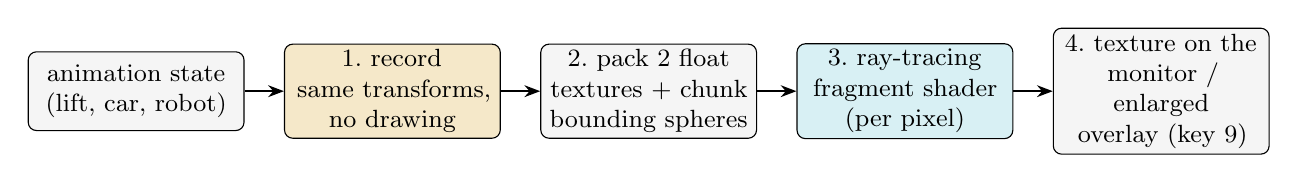
\begin{tikzpicture}[font=\small, node distance=5mm,
  st/.style={draw, rounded corners=3pt, fill=gray!8, minimum height=10mm, text width=26mm, align=center, inner sep=2pt},
  tc/.style={st, fill=smcyan!18},
  ta/.style={st, fill=smamber!25},
  arr/.style={-{Stealth[length=2mm]}, thick}]
  \node[st] (s0) {animation state\\(lift, car, robot)};
  \node[ta, right=of s0] (s1) {1.\ record\\same transforms,\\no drawing};
  \node[st, right=of s1] (s2) {2.\ pack 2 float\\textures + chunk\\bounding spheres};
  \node[tc, right=of s2] (s3) {3.\ ray-tracing\\fragment shader\\(per pixel)};
  \node[st, right=of s3] (s4) {4.\ texture on the\\monitor / enlarged\\overlay (key 9)};
  \foreach \a/\b in {s0/s1,s1/s2,s2/s3,s3/s4} \draw[arr] (\a) -- (\b);
\end{tikzpicture}
}
\caption{The four steps of the monitor pass (\fn{rtRender()} in \fn{Main.cpp}); the main garage renderer is unchanged.}\label{fig:rtpipe}
\end{figure}
\begin{enumerate}[leftmargin=*,label=\textbf{\arabic*.}]
\item \textbf{Record.} \fn{Scene::recordInspectionGeometry()} (SceneObjects.cpp) re-runs \fn{drawHydraulicLift()}, \fn{drawCar()} and
\fn{drawRobotArm()} in \emph{record mode}: \fn{drawCube}, \fn{drawCylinder}, \fn{drawSphere} and the car-shell batches append what they would have drawn --- with the \emph{same
matrices} --- to a list instead of drawing. The lift, the car (via \fn{serviceCarMatrix()}), the wheels (\fn{wheelSpin}) and the robot (all five joints and the fitted tool) therefore follow the live animation state with no second copy of the logic.
\item \textbf{Pack.} The list ($790$--$793$ items) is written into an RGBA32F texture, four texels per item, and sorted along a Morton (Z-order) curve of their centres and grouped into chunks of $16$ consecutive items, each with a bounding sphere.
\item \textbf{Trace.} A fullscreen fragment shader (\fn{kRayTraceFragmentShader}, \fn{Shader.cpp}) runs once per monitor pixel into an off-screen RGBA8 texture ($512{\times}320$, refreshed every second frame; $1024{\times}640$ every frame when enlarged).
\item \textbf{Display.} The texture is mapped on the monitor's screen quad inside the garage (\fn{rtDrawScreen()}) and, on key \fn{9}, drawn as a large overlay on top of the finished frame (\fn{rtDrawOverlay()}). The pass restores the framebuffer, viewport, program and enable-state it changes.
\end{enumerate}

\subsection{Ray generation}
For pixel coordinates $(u,v)\in[-1,1]^2$, aspect $a=512/320=1.6$ and vertical field of view $\varphi=64^\circ$ ($\tan\frac{\varphi}{2}=0.625$), the camera ray is
\begin{equation}\vect o=\vect c,\qquad \vect d=\operatorname{normalize}\Big(\vect f+u\,a\tan\tfrac{\varphi}{2}\,\vect r+v\tan\tfrac{\varphi}{2}\,\vect{u}\Big),\label{eq:rtray}\end{equation}
where $\vect c$ is the camera position and $(\vect f,\vect r,\vect u)$ its forward, right and up vectors (\fn{rtCamera()}). The camera looks at a point that rises with the lift,
$\vect T=(0,\;0.5\,y_{\text{top}}+0.45,\;-2)$ with $y_{\text{top}}=\fn{liftTopY}(h)$ (for the robot-side preset $\vect T=(-0.72,\;0.5\,y_{\text{top}}+0.52,\;-2.10)$), so raising the car changes the image.
Four presets (key \fn{=}, \fn{gRtPreset}, names in \fn{kRtPresetNames}) place the camera low beside or in front of the car:
\textbf{0} rear underbody $\vect c=(0.35,0.55,6.8)$; \textbf{1} nose underbody $(0.35,0.55,-9.0)$; \textbf{2} opposite-side overview $(5.4,0.75,-3.6)$; \textbf{3} \emph{live robot-side diagnostic} $(-5.75,0.78,-5.10)$.
Preset~3 is the \textbf{default}: it watches the same $-x$ flank that the robot services, so the arm, its tool, its shadow and the panel being worked on are all in view while the service runs. \fn{Insert}/\fn{Delete} orbit the camera about $\vect T$ (\fn{gRtYaw}); pressing \fn{=} resets the orbit.

\subsection{Intersections}
Each item is tested against the ray $\vect o+t\vect d$, $|\vect d|=1$. Boxes, cylinders and ellipsoids are the \emph{unit shapes} of the rasteriser (cube $[-\tfrac12,\tfrac12]^3$, cylinder $r=\tfrac12$, $y\in[-\tfrac12,\tfrac12]$, sphere $r=\tfrac12$)
placed by their model matrix $M$. The shader stores $M^{-1}$ and transforms the ray into the shape's own space, $\vect o'=M^{-1}\vect o$, $\vect d'=M^{-1}\vect d$ (not renormalised, so the same $t$ is valid in both spaces):
\begin{align}
\text{box:}\quad & t_{1,2}=\frac{\mp\frac12-o'}{d'}\ \text{(per axis)},\quad t_n=\max\min(t_1,t_2),\ t_f=\min\max(t_1,t_2),\ \text{hit iff } t_n\le t_f,\ t_f>0;\\
\text{cylinder:}\quad & a=d_x'^2+d_z'^2,\ b=o_x'd_x'+o_z'd_z',\ c=o_x'^2+o_z'^2-\tfrac14,\quad t=\frac{-b\mp\sqrt{b^2-ac}}{a},\ |o_y'+td_y'|\le\tfrac12,\ \text{plus caps } y=\pm\tfrac12;\\
\text{sphere:}\quad & |\vect o'+t\vect d'|^2=\tfrac14;\qquad
\text{triangle (M\"oller--Trumbore):}\quad t=\frac{\vect e_2\cdot(\vect s\times\vect e_1)}{\vect e_1\cdot(\vect d\times\vect e_2)},\ \vect s=\vect o-\vect a.
\end{align}
The world normal of a box, cylinder or sphere hit is $\vect n=\operatorname{normalize}\big((M^{-1})^{T}\vect n'\big)$; a triangle's is the normalised $\vect e_1\times\vect e_2$ (flipped to face the ray). The floor is the analytic plane $y=0$, $t=-c_y/d_y$.

\subsection{Nearest hit, shading and the shadow ray}
\textbf{Nearest surface.} The tracer keeps the smallest valid $t$ found so far (\fn{tBest}); every later candidate must beat it (\fn{hitItem(\dots,tBest,\dots)}), so a farther surface can never replace a nearer one. The object hit is compared with the floor distance the same way.
Before looking inside a chunk, the ray is tested against the chunk's bounding sphere; a chunk that the ray misses, or whose nearest possible point lies beyond \fn{tBest}, is skipped.

\textbf{Shading and shadow ray.} At the hit point $P$ with normal $\vect n$ (flipped to face the viewer) and material colour $\vect k$ (the colour of the primitive the rasteriser uses), the inspection light at $P_L$ --- one of five presets in \fn{kRtLights} (key \fn{PageDown}); the default (index 2) is a floor lamp on the robot side at $(-2.6,\,0.6,\,-6.0)$, and the numpad moves it freely --- gives
\begin{equation}I=\vect k\Big(0.085+0.06\,n_y+0.05\max(\vect n\!\cdot\!\vect V,0)\Big)+A\,v\Big[\vect k\max(\vect n\!\cdot\!\vect L,0)+0.30\max(\vect n\!\cdot\!\vect H,0)^{48}\Big],\qquad A=\frac{4.6}{1+0.10\,d+0.04\,d^2},\ d=|P_L-P|,\label{eq:rtshade}\end{equation}
and an exposure curve $1-e^{-1.35I}$ with gamma $1/2.2$. The visibility $v$ comes from a \textbf{shadow ray}: origin $P+0.012\,\vect n$ (to avoid hitting its own surface), direction $\vect L=(P_L-P)/d$ and
\begin{equation}t_{\max}=d-0.03,\qquad v=\begin{cases}0&\text{if any item has a hit with }0<t<t_{\max}\\1&\text{otherwise,}\end{cases}\label{eq:rtshadow}\end{equation}
so only blockers \emph{between} the surface and the light count; anything behind the light is ignored (Fig.~\ref{fig:rtpath}). When shadow rays are switched off (key \fn{-}) the same ray, camera, geometry, colours and light give $v=1$, which is the comparison of Fig.~\ref{fig:rtshadow}.
\begin{figure}[!htbp]\centering
\resizebox{0.96\textwidth}{!}{% Ray path of the inspection monitor: primary ray, nearest hit, shadow ray (blocked by a robot link; a blocker beyond the light is ignored).
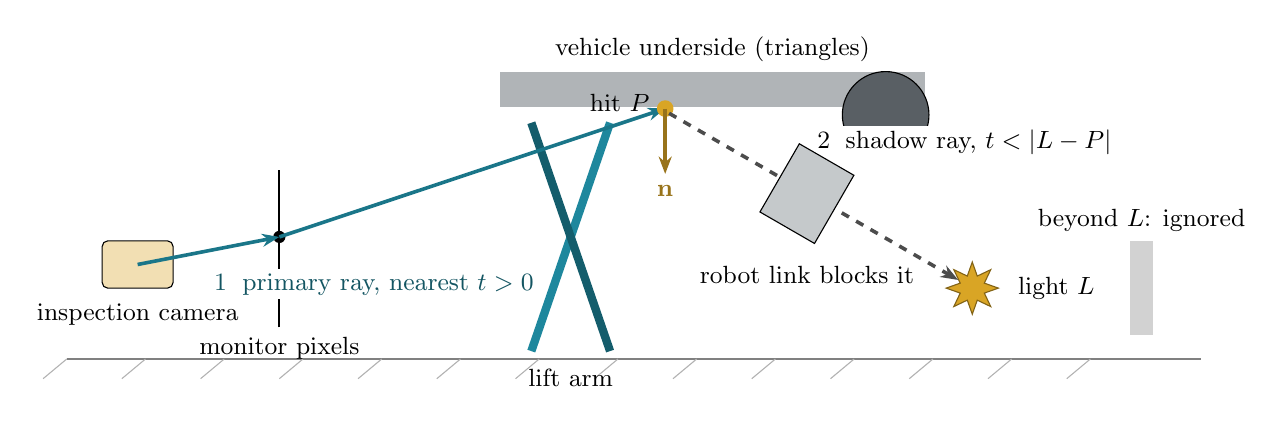
\begin{tikzpicture}[x=1cm,y=1cm,font=\small,
  arr/.style={-{Stealth[length=2.2mm]}, line width=1.3pt},
  lbl/.style={fill=white, inner sep=1.5pt}]
  % floor
  \draw[gray, line width=1pt] (-0.5,0) -- (13.9,0);
  \foreach \x in {0,1,...,13} \draw[gray!60] (\x-0.5,0) -- (\x-0.8,-0.25);
  % car underside + wheel
  \fill[smsteel!55] (5.0,3.2) rectangle (10.4,3.65);
  \node[above] at (7.7,3.65) {vehicle underside (triangles)};
  \draw[fill=smsteel!80!black] (9.9,3.1) circle (0.55);
  % lift stack
  \draw[line width=3pt, smcyan!80!black] (5.4,0.1) -- (6.4,3.0);
  \draw[line width=3pt, smcyan!55!black] (6.4,0.1) -- (5.4,3.0);
  \node[below] at (5.9,0) {lift arm};
  % camera and image plane
  \node[draw, fill=smamber!35, rounded corners=2pt, minimum width=0.9cm, minimum height=0.6cm] (cam) at (0.4,1.2) {};
  \node[below=2pt] at (cam.south) {inspection camera};
  \draw[thick] (2.2,0.4) -- (2.2,2.4);
  \node[below] at (2.2,0.4) {monitor pixels};
  \fill (2.2,1.55) circle (2.2pt);
  % primary ray
  \draw[arr, smcyan!70!black] (0.4,1.2) -- (2.2,1.55);
  \draw[arr, smcyan!70!black] (2.2,1.55) -- (7.1,3.18);
  \node[lbl, text=smcyan!50!black] at (3.4,0.95) {1\; primary ray, nearest $t>0$};
  \fill[smamber] (7.1,3.18) circle (3pt);
  \node[above left=1pt] at (7.05,3.0) {hit $P$};
  \draw[arr, smamber!70!black] (7.1,3.18) -- (7.1,2.35) node[below] {$\mathbf n$};
  % light and shadow ray
  \node[star, star points=8, star point ratio=2.0, fill=smamber, draw=smamber!60!black, minimum size=0.55cm] (L) at (11.0,0.9) {};
  \node[right=3pt] at (L.east) {light $L$};
  \draw[arr, dashed, black!70] (7.15,3.12) -- (L);
  \node[lbl] at (10.9,2.75) {2\; shadow ray, $t<|L-P|$};
  % blocker between (robot link)
  \draw[fill=smsteel!40, rotate around={-30:(8.9,2.1)}] (8.5,1.6) rectangle (9.3,2.6);
  \node[below] at (8.9,1.3) {robot link blocks it};
  % blocker beyond the light (ignored)
  \fill[gray!35] (13.0,0.3) rectangle (13.3,1.5);
  \node[above] at (13.15,1.5) {beyond $L$: ignored};
\end{tikzpicture}
}
\caption{Ray path: (1) the camera ray through a monitor pixel finds the nearest hit $P$ on the underside; (2) a shadow ray runs from $P$ toward the light $L$; a robot link between them blocks it (shadow), a blocker beyond $L$ is ignored.}\label{fig:rtpath}
\end{figure}

\subsection{What is traced, acceleration structure and approximations}
\begin{table}[!htbp]\centering\scriptsize
\caption{Contents of the traced scene at the default state (lift raised, robot at the tool station; counts printed by the program with \fn{--capture}).}\label{tab:rtscene}
\begin{tabular}{@{}l l r@{}}\toprule
Object & Traced as & Items\\\midrule
Hydraulic lift (base, scissor arms, pins, rams, runways) & boxes, cylinders (the lift's own primitives) & $114$\\
Serviced vehicle: underbody, side skin, arches, bumpers, trim & triangles of the car-shell batches (glass and lamps omitted) & $452$\\
Vehicle wheels and detail parts & cylinders and boxes of \fn{drawWheel()} and \fn{drawCar()} & $184$\\
Robot arm and the fitted tool & boxes, cylinders, spheres of \fn{drawRobotArm()} & $41$--$43$\\
Floor & analytic plane $y=0$ & --\\\midrule
\textbf{Total} & & $\mathbf{793}$ ($50$ chunks of $16$)\\\bottomrule
\end{tabular}
\end{table}
\textbf{Acceleration structure.} A one-level bounding-volume hierarchy: consecutive items (which are spatially close, because they are drawn part by part) form chunks of 16 (after Morton sorting) with a bounding sphere computed on the CPU every frame. A ray visits a chunk's items only if it enters the sphere. With $\approx790$ items this gives an interactive monitor on an OpenGL~3.3 GPU; a deeper BVH would be needed for much larger scenes. \textbf{Measured cost} (integrated Intel Iris Xe, capture frame with \fn{glFinish}): about $25$~ms for the $512{\times}320$ monitor image and about $45$~ms for the enlarged $1024{\times}640$ view, which is why the small monitor refreshes every second frame; a dedicated GPU is faster.\\
\textbf{Documented approximations.} The monitor is \emph{not} an exact copy of the visible garage: (i) the car is its shell triangles without glass or lamps; (ii) details smaller than $6$~cm (bolts, rivets) are dropped; (iii) the turntable plate, hoses, tool station and the rest of the building are not traced, so the underside of the car is visible; (iv) the floor is a plane with painted grid lines; (v) there is one light, one shadow ray and no reflections or global illumination. The vehicle components shown are exactly those the project models --- none are invented.

\subsection{Controls}
\begin{table}[!htbp]\centering\scriptsize
\caption{Inspection-monitor controls (keys checked against the existing bindings; all are new).}\label{tab:rtkeys}
\begin{tabular}{@{}>{\raggedright}p{3.2cm}>{\raggedright}p{6.4cm}>{\raggedright\arraybackslash}p{5.2cm}@{}}\toprule
Key & Action & Variable\\\midrule
\fn{9} & enlarge / close the inspection view (re-renders at $1024{\times}640$) & \fn{gRtLarge}\\
\fn{-} & inspection-light shadow rays on / off & \fn{gRtShadows}\\
\fn{=} & next camera preset (rear, nose, opposite side, robot side = default) & \fn{gRtPreset}\\
\fn{Insert} / \fn{Delete} & orbit the inspection camera & \fn{gRtYaw}\\
\fn{PageDown} & next light position (5 presets; default: robot-side floor lamp) & \fn{gRtLightIdx}\\
Numpad \fn{4 6 8 2 + -} & move the inspection light freely (x, z, height) & \fn{gRtLight}\\\bottomrule
\end{tabular}
\end{table}
Command-line switches for repeatable figures: \fn{--rtfull}, \fn{--rtlarge}, \fn{--rtpreset}, \fn{--rtshadow}, \fn{--rtlight x y z}, \fn{--rtlightidx}, \fn{--rtyaw}. The existing keys, shading modes, lighting, car, lift, robot and the 18-state service are unchanged.

\subsection{Results and verification}
\begin{figure}[!htbp]\centering
\begin{subfigure}{0.32\textwidth}\shot{\linewidth}{images/raytrace/l0.jpg}\caption{lift down, $h=0$}\end{subfigure}\hfill
\begin{subfigure}{0.32\textwidth}\shot{\linewidth}{images/raytrace/l1.jpg}\caption{$h=1.10$ (service height)}\end{subfigure}\hfill
\begin{subfigure}{0.32\textwidth}\shot{\linewidth}{images/raytrace/l2.jpg}\caption{$h=2.50$}\end{subfigure}
\caption{Raising the car changes the traced image: the scissor stack opens, the car rises and the camera follows the raised target.}\label{fig:rtlift}
\end{figure}
\begin{figure}[!htbp]\centering
\begin{subfigure}{0.49\textwidth}\shot{\linewidth}{images/raytrace/on.jpg}\caption{shadow rays on}\end{subfigure}\hfill
\begin{subfigure}{0.49\textwidth}\shot{\linewidth}{images/raytrace/off.jpg}\caption{shadow rays off}\end{subfigure}
\caption{Same robot-side camera, geometry, colours and light (light preset 3 at $(3.4,2.6,-2)$, state at $t=110$ s, polishing): only $v$ of Eq.~\eqref{eq:rtshadow} changes. With shadows on, the scissor lift and the car cast their shadow across the floor.}\label{fig:rtshadow}
\end{figure}
\begin{figure}[!htbp]\centering
\begin{subfigure}{0.32\textwidth}\shot{\linewidth}{images/raytrace/t30.jpg}\caption{$t=30$ s, scanning}\end{subfigure}\hfill
\begin{subfigure}{0.32\textwidth}\shot{\linewidth}{images/raytrace/t110.jpg}\caption{$t=110$ s, polishing}\end{subfigure}\hfill
\begin{subfigure}{0.32\textwidth}\shot{\linewidth}{images/raytrace/t154.jpg}\caption{$t=154$ s, wheel service}\end{subfigure}\\[2pt]
\begin{subfigure}{0.32\textwidth}\shot{\linewidth}{images/raytrace/g30.jpg}\caption{garage view, $t=30$ s}\end{subfigure}\hfill
\begin{subfigure}{0.32\textwidth}\shot{\linewidth}{images/raytrace/g110.jpg}\caption{garage view, $t=110$ s}\end{subfigure}\hfill
\begin{subfigure}{0.32\textwidth}\shot{\linewidth}{images/raytrace/g154.jpg}\caption{garage view, $t=154$ s}\end{subfigure}
\caption{Synchronisation: the traced monitor in its default robot-side view (top) and the garage seen from the robot side (bottom) at the same simulation times; the robot arm, its tool and the turntable-rotated car match.}\label{fig:rtsync}
\end{figure}
\begin{table}[!htbp]\centering\scriptsize
\caption{Verification performed with the final build.}\label{tab:rtverify}
\begin{tabular}{@{}>{\raggedright}p{4.0cm}>{\raggedright}p{6.9cm}>{\raggedright\arraybackslash}p{3.9cm}@{}}\toprule
Check & How & Result\\\midrule
Raising the car changes the image & captures at $h=0,\,1.10,\,2.50$ (Fig.~\ref{fig:rtlift}) & scissor opens, car rises: passed\\
Wheels and robot synchronised & monitor and garage captured at $t=30,110,154$ s (Fig.~\ref{fig:rtsync}) & arm, tool, car yaw match: passed\\
Nearest surface hides what is behind & wheels and arches hide the lift behind them in the robot-side view; \fn{tBest} logic & passed (visual and code)\\
Shadow rays only use blockers before the light & $t_{\max}=d-0.03$; blockers beyond the light have no effect & passed (code; Fig.~\ref{fig:rtpath})\\
Same scene with shadows on/off & identical capture arguments except \fn{--rtshadow} (Fig.~\ref{fig:rtshadow}) & only the shadows differ: passed\\
Enlarge / close & \fn{--rtlarge}, overlay at $1024{\times}640$ (Fig.~\ref{fig:rtroom}b) & passed\\
Existing service still runs & \fn{--simtime} to $154$ s and the full $197.7$ s sequence reach COMPLETE & passed\\
Builds & x64 Release and Debug & no errors, no compiler warnings\\
\textbf{Not performed} & live interactive key presses in a window, other GPUs, shader-failure fault injection (the failure path returns before any monitor state is used) & stated honestly\\\bottomrule
\end{tabular}
\end{table}
\viva{Ray-traced inspection monitor}{\fn{Shader.cpp}, \fn{Main.cpp}, \fn{SceneObjects.cpp}}{\fn{kRayTraceFragmentShader} (\fn{hitItem}, \fn{traceClosest}, \fn{occluded}), \fn{rtRender()}, \fn{rtCamera()}, \fn{Scene::recordInspectionGeometry()}, \fn{Scene::inspectionMonitorMatrix()}}
{$\varphi=64^\circ$; $512{\times}320$ / $1024{\times}640$; default preset 3 (robot side), light index 2; chunk size $16$; light power $4.6$; shadow bias $0.012$; $t_{\max}=d-0.03$; $793$ items; monitor at $(4.4,0,-5.6)$, screen $2.0{\times}1.25$ m}
{a larger chunk size (16 now) tests fewer spheres but more items per hit; raising the light power brightens the picture; a larger bias removes self-shadowing at grazing angles but detaches shadows; more items (a less aggressive size cut-off, 6 cm) slows the pass; \fn{-} removes the shadow term.}
{Eqs.~\eqref{eq:rtray}--\eqref{eq:rtshadow}; Figs.~\ref{fig:rtpipe}--\ref{fig:rtsync}}

% =====================================================================
\section{Motion, Animation, Interaction and Collision}\label{sec:motion}
\textbf{Interpolation.} Door, lift and drive use constant-speed \fn{moveToward()}: $p\leftarrow p+\operatorname{clamp}(p_1-p,\pm v\Delta t)$.
Robot moves share one eased timeline (\fn{moveRobotTowardPose()}):
\begin{equation}u=\min\!\big(t/T,1\big),\;s(u)=3u^2-2u^3,\;\theta_j(t)=\theta_j^0+s(u)\,\text{wrap}_{180}(\theta_j^1-\theta_j^0),\;
T=\max\!\Big(0.22,\tfrac{\max_j|\Delta_j|}{52k}\Big),\label{eq:smooth}\end{equation}
i.e.\ $p(t)=(1-s)p_0+sp_1$ with zero speed at both ends; wrapping takes the short way ($170^\circ\to-170^\circ$ is $+20^\circ$).

\textbf{Vehicle and wheels.} \fn{carDrive} changes at 0.092/s, so the \SI{18.5}{m} run takes \SI{10.87}{s} (\SI{1.70}{m/s}). The ramp is
sampled under each axle (Eq.~\eqref{eq:ramp}, Fig.~\ref{fig:door}). Rolling without slipping:
\begin{equation}\Delta\phi_{\deg}=\frac{\Delta s}{r}\frac{180}{\pi}\;\Rightarrow\;\phi_{\text{run}}=\frac{18.5}{0.450}\frac{180}{\pi}=2355.5^\circ=6.54\text{ turns}.\label{eq:roll}\end{equation}

\textbf{Everything that moves} (variable, rate): vehicle \fn{carDrive} $0.092$/s (Eq.~\eqref{eq:car}); wheels \fn{wheelSpin} (Eq.~\eqref{eq:roll}); door \fn{gDoorOffset} $0.8$ m/s;
lift \fn{gLiftHeight} $0.55$ m/s; robot joints Eq.~\eqref{eq:smooth} at $52^\circ$/s; turntable \fn{carYaw} $34^\circ$/s the short way; polisher pad $620^\circ$/s and impact-driver socket $980^\circ$/s;
gripper opening $1.8$--$2.4$/s and lug nuts $1.35$/s (they seat $30$ mm); warning beacon $0.35+0.65(\tfrac12+\tfrac12\sin9t)$ while the door moves.

\textbf{Interaction.} Discrete keys are
edge-detected once per press (e.g.\ \fn{F5}: \fn{gShadingMode = (gShadingMode + 1) \% 3}); held keys change a value every frame and are
validated by \fn{robotPoseSafe()} before being applied (Table~\ref{tab:keys}).
\begin{table}[!htbp]\centering\scriptsize
\caption{Controls grouped by feature (verified against \fn{handleDiscreteKey()} and \fn{processMovement()} in \fn{Main.cpp}).}\label{tab:keys}
\begin{tabular}{@{}>{\raggedright}p{3.3cm}>{\raggedright}p{4.3cm}>{\raggedright}p{3.7cm}>{\raggedright\arraybackslash}p{3.7cm}@{}}\toprule
Input & Action & Variable / function & Visible effect\\\midrule
\multicolumn{4}{@{}l}{\textbf{CAMERA}}\\
\fn{W A S D}, \fn{Space}/\fn{Ctrl} (\fn{E}/\fn{Q}), \fn{Shift} & move (\SI{7}{m/s}, $\times2.5$ with Shift) & \fn{gCamera.position} & fly through the garage\\
Mouse, scroll, \fn{Tab} & look, zoom (FOV 20--90$^\circ$), free the cursor & \fn{yaw, pitch, fov} & view direction and zoom\\
\multicolumn{4}{@{}l}{\textbf{DOOR, LIFT AND VEHICLE}}\\
\fn{O}; \fn{Z}/\fn{X}/\fn{C} & door auto toggle; close / open / stop & \fn{gDoorTarget}, \fn{gDoorOffset} & roller door moves\\
\fn{P}; \fn{[} \fn{]} \fn{\textbackslash} & lift auto (3.20 / down); lower / raise / stop & \fn{gLiftTarget}, \fn{gLiftHeight} & lift moves (collision-checked)\\
\fn{Home}; \fn{PgUp} & vehicle out / in; back to the apron & \fn{gCarDriveTarget} & vehicle drives\\
\multicolumn{4}{@{}l}{\textbf{ROBOT}}\\
\fn{T/G}, \fn{U/J}, \fn{I/K}, \fn{Y/H}, $\leftarrow/\rightarrow$ & base yaw, shoulder, elbow, wrist pitch, wrist roll & Fig.~\ref{fig:robot} & arm and spotlight move\\
\fn{F1}--\fn{F4} & scanner / driver / gripper / polisher & \fn{gRobotTool} & tool head changes\\
\multicolumn{4}{@{}l}{\textbf{LIGHTING}}\\
\fn{;}, \fn{'}, \fn{/}, \fn{End} & ceiling lights, headlights, neon, beacon & \fn{gSwitches.*} & lights switch\\
\fn{0} & outside light: daylight $\leftrightarrow$ night & \fn{gNight}, \fn{applyDayNight()} & blue sky and sun / dark sky and dim moon\\
\fn{M}; \fn{,} \fn{.} & lighting preset; reflection (IBL) intensity & \fn{gLightingPreset}, \fn{gIblIntensity} & whole rig / reflections change\\
\multicolumn{4}{@{}l}{\textbf{INSPECTION MONITOR (ray tracing)}}\\
\fn{9}, \fn{-}, \fn{=} & enlarge/close; shadow rays on/off; camera preset & \fn{gRtLarge}, \fn{gRtShadows}, \fn{gRtPreset} & monitor image changes (Section~\ref{sec:rt})\\
\fn{Insert/Delete}, \fn{PageDown}, numpad & orbit camera; light preset; move light & \fn{gRtYaw}, \fn{gRtLightIdx}, \fn{gRtLight} & view and shadows change\\
\multicolumn{4}{@{}l}{\textbf{SHADING AND PROJECTION}}\\
\fn{F5} & PBR $\to$ Gouraud $\to$ Phong & \fn{gShadingMode} & shading model changes\\
\fn{F6}--\fn{F11} & textures, bump, shadows, reflections, bloom, MSAA & \fn{gTexturesEnabled} \dots & feature on / off\\
\fn{Backspace} & perspective / orthographic & \fn{gOrthographic} & projection changes\\
\multicolumn{4}{@{}l}{\textbf{AUTOMATIC SERVICE, DEBUG AND TEACHING}}\\
\fn{Enter}, \fn{R} & start / reset the automatic service & \fn{startServiceDemo()} & full sequence (Section~\ref{sec:fsm})\\
\fn{L}, \fn{1}--\fn{8}, \fn{N}/\fn{B}, \fn{V}, \fn{F}, \fn{F12} & wireframe, isolate object, build stage, report, screenshot, orbit & various & teaching and demo aids\\\bottomrule
\end{tabular}
\end{table}

\textbf{Collision.} The arm is three swept segments (shoulder$\to$elbow, elbow$\to$wrist, wrist$\to$tool tip; radii 0.20, 0.18,
0.22--0.28\,m) tested against AABBs inflated by the radius (slab test, \fn{segmentHitsAABB()}: per axis $t_{1,2}=(b_{\min,\max}-a)/d$, hit iff $\max_{\text{axes}}\min(t_1,t_2)\le\min_{\text{axes}}\max(t_1,t_2)$ within the segment); boxes overlap iff
$A_{\min}\le B_{\max}\wedge A_{\max}\ge B_{\min}$ on every axis~\cite{ericson2005collision}. Checked: pedestal, tool table, other lifts,
power pack, ramp, ceiling fixtures, main lift, turntable disc and the vehicle (AABB of the rotated footprint,
$h_x=|\cos\psi|1.34+|\sin\psi|2.95$). In service mode the tool may approach the paint but never enter the solid
shell/wheel boxes; a blocked manual move is rejected and the title shows ``SAFETY STOP''. \emph{Example}
(\fn{POSE\_LUG\_1}, $h=1.10$): the driver tip is at $x=-1.305$ and the inflated wheel box starts at $x=-1.25$, giving \SI{55}{mm}
clearance, so contact is allowed.
\viva{Collision safety}{\fn{Main.cpp}}{\fn{robotPoseSafe()}, \fn{segmentHitsAABB()}, \fn{segmentSegmentDistance()}, \fn{liftPositionSafe()}}
{segment radii 0.20/0.18/0.28; vehicle solid $x\in[-1.03,1.03]$, $y\in[y_t{+}0.28,\,y_t{+}1.80]$; wheels $|x|\le1.24$; margin 0.010; workspace $0.18\le y\le6.72$}
{larger radii make the arm stop earlier (more conservative); shrinking a box lets the tool approach closer; setting \fn{allowVehicleServiceContact}=false keeps the tool out of the whole approach volume.}
{slab test; overlap condition above}

% =====================================================================
\section{Automatic Service Workflow}\label{sec:fsm}
\fn{updateServiceAutomation(dt)} switches on \fn{gServiceState}; each state advances \fn{gServicePhase} when its completion
condition holds (Fig.~\ref{fig:fsm}; times measured with the fixed-step \fn{--simtime} capture mode). Every state has the same shape: set targets, wait for the completion condition, call \fn{setServiceState()}.
\begin{figure}[!htbp]\centering
\resizebox{0.98\textwidth}{!}{% ServiceState sequence from updateServiceAutomation(); start times measured with --simtime (speed 1.0).
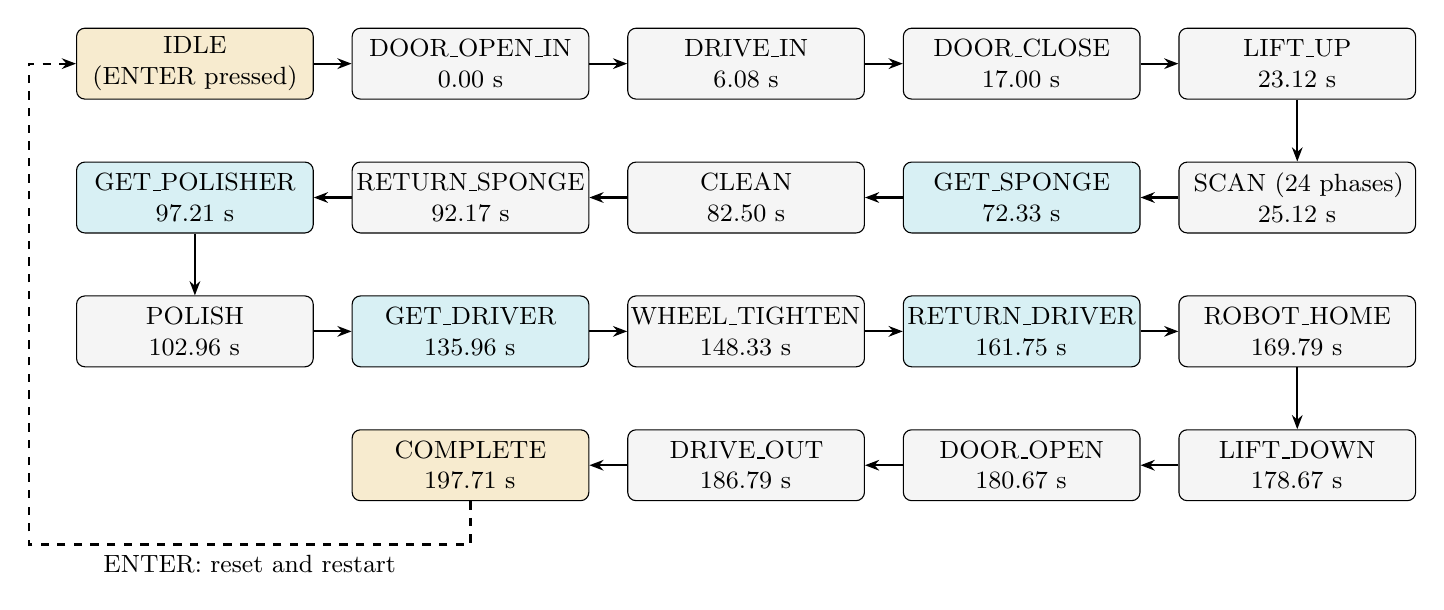
\begin{tikzpicture}[
  font=\small,
  st/.style={draw, rounded corners=3pt, fill=gray!8, minimum height=9mm,
             text width=29mm, align=center, inner sep=1.5pt},
  tc/.style={st, fill=smcyan!18},
  arr/.style={-{Stealth[length=1.8mm]}, thick}]
  \def\dx{3.5}
  \node[st, fill=smamber!22] (s0) at (0,0)        {IDLE\\ (ENTER pressed)};
  \node[st] (s1) at (1*\dx,0)  {DOOR\_OPEN\_IN\\ 0.00 s};
  \node[st] (s2) at (2*\dx,0)  {DRIVE\_IN\\ 6.08 s};
  \node[st] (s3) at (3*\dx,0)  {DOOR\_CLOSE\\ 17.00 s};
  \node[st] (s4) at (4*\dx,0)  {LIFT\_UP\\ 23.12 s};
  \node[st] (s5) at (4*\dx,-1.7) {SCAN (24 phases)\\ 25.12 s};
  \node[tc] (s6) at (3*\dx,-1.7) {GET\_SPONGE\\ 72.33 s};
  \node[st] (s7) at (2*\dx,-1.7) {CLEAN\\ 82.50 s};
  \node[st] (s8) at (1*\dx,-1.7) {RETURN\_SPONGE\\ 92.17 s};
  \node[tc] (s9) at (0,-1.7)     {GET\_POLISHER\\ 97.21 s};
  \node[st] (s10) at (0,-3.4)      {POLISH\\ 102.96 s};
  \node[tc] (s11) at (1*\dx,-3.4)  {GET\_DRIVER\\ 135.96 s};
  \node[st] (s12) at (2*\dx,-3.4)  {WHEEL\_TIGHTEN\\ 148.33 s};
  \node[tc] (s13) at (3*\dx,-3.4)  {RETURN\_DRIVER\\ 161.75 s};
  \node[st] (s14) at (4*\dx,-3.4)  {ROBOT\_HOME\\ 169.79 s};
  \node[st] (s15) at (4*\dx,-5.1)  {LIFT\_DOWN\\ 178.67 s};
  \node[st] (s16) at (3*\dx,-5.1)  {DOOR\_OPEN\\ 180.67 s};
  \node[st] (s17) at (2*\dx,-5.1)  {DRIVE\_OUT\\ 186.79 s};
  \node[st, fill=smamber!22] (s18) at (1*\dx,-5.1) {COMPLETE\\ 197.71 s};
  \foreach \a/\b in {s0/s1,s1/s2,s2/s3,s3/s4,s4/s5,s5/s6,s6/s7,s7/s8,s8/s9,s9/s10,s10/s11,s11/s12,s12/s13,s13/s14,s14/s15,s15/s16,s16/s17,s17/s18}
     \draw[arr] (\a) -- (\b);
  \draw[arr, dashed] (s18.south) -- ++(0,-0.55) -| node[pos=0.25, below]{ENTER: reset and restart}
        ($(s0.west)+(-0.6,0)$) -- (s0.west);
\end{tikzpicture}
}
\caption{Automatic service state machine (18 states, \SI{197.7}{s}); blue states perform the visible 10-phase tool exchange (\fn{runToolChange()}).}\label{fig:fsm}
\end{figure}
\textbf{Completion conditions (all in \fn{Main.cpp}).} DOOR\_OPEN\_IN: \fn{gDoorOffset}$\ge4.80$; DRIVE\_IN: \fn{carDrive}$\le0.002$;
DOOR\_CLOSE: door $\le0.035$; LIFT\_UP: $|h-1.10|<0.025$; SCAN: 24 pose phases (6 regions, turntable $180^\circ$ and back);
GET\_SPONGE / GET\_POLISHER / GET\_DRIVER: the 10-phase tool exchange; CLEAN: \fn{dirtAmount} $1\to0$ in 3 wiping bands;
POLISH: \fn{polishAmount} $0\to1$ (16 phases, both flanks); WHEEL\_TIGHTEN: star order 1-3-5-2-4 with \fn{lugProgress[i]};
ROBOT\_HOME: HOME pose reached; LIFT\_DOWN: $h\le0.025$; DOOR\_OPEN; DRIVE\_OUT: \fn{carDrive}$\ge0.998$ $\to$ COMPLETE.

% =====================================================================
\section{Requirement Fulfilment and Final Verification}\label{sec:audit}
\par\noindent\fcolorbox{smcyan}{smcyan!5}{\begin{minipage}{\dimexpr\linewidth-2\fboxsep-2\fboxrule\relax}\small
\textbf{FINAL VERIFICATION.}\;
\textbf{Proposal completion:} 21\,/\,21 (Table~\ref{tab:proposal}) \;\;|\;\;
\textbf{Mandatory requirements:} Lighting \checkmark\; Transformation \checkmark\; Gouraud \checkmark\; Phong \checkmark\; Motion \checkmark\; Interaction \checkmark \;\;|\;\;
\textbf{Build:} x64 Debug \checkmark\; Release \checkmark\ (no errors; the only messages are linker notices that \fn{glfw3.lib} ships without debug symbols).
Values in this report were read from the source constants; every scene figure was rendered by the final build. The inspection monitor is ray traced (Section~\ref{sec:rt}); the rest of the garage is rasterised, and no ray tracing is claimed for it.
\end{minipage}}\par

% =====================================================================
\section{Conclusion}\label{sec:conc}
All 21 proposal items and all six mandatory requirements are implemented and can be shown live; PBR, shadows, textures, HDR, the tool-exchange service and the ray-traced inspection monitor (bonus) go beyond the proposal.

\textbf{Technical references and development sources.} The theory follows the cited OpenGL~3.3 and GLSL specifications, \emph{Learn OpenGL},
Phong (1975), Gouraud (1971), Blinn (1977), Cook--Torrance (1982), GGX/Smith/Schlick, the UE4 and Disney shading courses, the ACES fit and
Ericson's collision text. The only third-party code is GLFW (window and input) and GLAD (OpenGL loader), bundled in \fn{Libraries/} and
\fn{glad.c}; the project loads no model or image files --- meshes, textures and shaders are generated by the six project source files
(\fn{Math3D.h}, \fn{Camera.h}, \fn{Primitives.cpp}, \fn{SceneObjects.cpp}, \fn{Shader.cpp}, \fn{Main.cpp}).

\begingroup\scriptsize\setlength{\itemsep}{0pt}\setlength{\parskip}{0pt}
\renewcommand{\section}[2]{\par\smallskip\textbf{#2}\par}
\bibliographystyle{ieeetr}
\bibliography{references}\endgroup
\end{document}
